\chapter{Experimental Results}
\label{ch:experimental-results}
This chapter, by exploring the complex design space of spatial accelerators, seeks to quantify the performance, energy, and memory trade-offs inherent in layer fusion. The investigation evaluate modified versions of the DepFiN and Eyeriss architectures across a diverse set of convolutional neural network workloads.

The chapter is organized into three main parts. First, the experimental setup is detailed, defining the selected hardware architectures, the targeted activation and weight-dominant workloads, and the comparative evaluation scenarios. 

\section{Experimental Setup}

This section details the methodology and configurations used to evaluate the scheduling of multiple fused layers. Accordingly, Section~\ref{sec:architectures} first defines the spatial architectures modeled in this study, specifically, modified variants of the DepFiN and Eyeriss~v1 accelerators adapted for multi-layer execution. Next, Section~\ref{sec:workloads} introduces the selected CNN workloads, covering both activation-dominant and weight-dominant networks to stress different aspects of the memory hierarchy. Finally, Section~\ref{sec:partial-full-fusion} outlines the evaluation scenarios, establishing a comparative framework between full fusion, partial fusion, and standard single-layer execution.

% ============================================================
%  N.1.1  Architectures
% ============================================================
\subsection{Architectures}
\label{sec:architectures}

The two spatial architectures selected for the experiments are
DepFiN~\cite{goetschalckx2023depfin} and Eyeriss~v1~\cite{eyeriss}.
Table~\ref{tab:orig-arch-comparison} summarizes the key parameters of the
\emph{original} designs as published in the respective papers.


\begin{table}[htbp]
  \centering
  \caption{Comparison of the original DepFiN and Eyeriss~v1 architectures.}
  \footnotesize
  \setlength{\tabcolsep}{4pt} % Reduced horizontal padding
  \renewcommand{\arraystretch}{0.95} % Slightly tighter vertical row spacing
  \label{tab:orig-arch-comparison}
  \small
  \begin{tabular}{l l l}
    \toprule
    \textbf{Parameter}          & \textbf{DepFiN}                      & \textbf{Eyeriss v1}                 \\
    \midrule
    Technology node              & 12\,nm                               & 65\,nm                              \\
    Clock frequency              & $\sim$930\,MHz                       & 200\,MHz                            \\
    Dataflow                     & Depth-first (output-stationary)      & Row-stationary                      \\
    PE array                     & $16 \times 128 = 2048$               & $12 \times 14 = 168$                \\
    \addlinespace
    On-chip memory               & Split FMEM + WMEM                    & Unified GlobalBuffer                \\
    FMEM / GlobalBuffer size     & 1056\,KB                             & 128\,KB                             \\
    WMEM size                    & 524\,KB                              & ---                                 \\
    \addlinespace
    PE registers                 & WeightReg (384),                     & InputSpad (24),                     \\
                                 & InputReg (24),                       & WeightSpad (384),                   \\
                                 & AccumulationReg (32)                 & PsumSpad (32)                       \\
    Accumulator precision        & 32\,bit                              & 16\,bit                             \\
    \addlinespace
    DRAM type                    & LPDDR4                               & LPDDR4                              \\
    DRAM bandwidth               & 12\,B/cycle                          & 8\,B/cycle                          \\
    FMEM read bandwidth          & 132\,B/cycle                         & ---                                 \\
    GB bandwidth                 & ---                                  & 32\,B/cycle                         \\
    \addlinespace
    Spatial mapping (cols)       & Output width ($Q$)                   & Output width ($Q$) + channels ($M$) \\
    Spatial mapping (rows)       & Output channels ($M$)                & Filter ($S$) + channels ($C$, $M$)  \\
    \bottomrule
  \end{tabular}
\end{table}

Both architectures were modeled in our model based on the
parameters published in~\cite{goetschalckx2023depfin,eyeriss}.
However, because the spatial architectures must support a variety of fused CNN
workloads, not only the single layer, several modifications were necessary.
We therefore refer to the modified variants as \textbf{DepFiN-Like} and
\textbf{Eyeriss-Like} throughout this chapter.

% ------------------------------------------------------------------
\subsubsection{DepFiN-Like}
\label{sec:depfin-like}

DepFiN is a depth-first CNN accelerator with a split on-chip memory
hierarchy: a \emph{Feature Memory} (FMEM) that stores input and output
activations while bypassing weights, and a \emph{Weight Memory} (WMEM) that
stores weights while bypassing all activation operands.
In fused (multi-layer) mode, intermediate activations between consecutive
layers are kept entirely on-chip, DRAM bypasses the intermediate operands
(\texttt{int\_in}, \texttt{int\_out}), so that inter-layer data never touches external memory (see Section \ref{sec:val-arch-extraction} for further details).
Each fused layer receives its own pair of spatial fanout levels (see Section \ref{sec:bg-sa-abstraction}): Systolic Array Columns (\texttt{SACols}) distributes the output spatial width ($Q$ or $X_i$) across
the PE columns, while Systolic Array Rows (\texttt{SARows}) distributes the output channels
($M$ or $Z_i$) across the PE rows.

Compared with the original DepFiN design the following modifications were applied:

\begin{enumerate}
  \item \textbf{Configurable tile size.}
        The original DepFiN fixes the output tile to a $1 \times 128$
        pixel patch that fills the 128 PE columns exactly.
        Our version relaxes this constraint, allowing the output tile
        size to be set independently for each workload.
        This is essential for exploring the effect of tile size on
        energy, latency, and DRAM traffic across workloads with
        different spatial dimensions (see Section~\ref{sec:cs1-tile}).

  \item \textbf{Variable PE array dimensions.}
        Instead of the fixed $16 \times 128$ array,
        we explore which results would give a different aspect ratios at a constant total PE count (Section~\ref{sec:cs4-aspect}).

  \item \textbf{Mapping.}
        The depth-first dataflow is preserved: weights are loaded into
        WMEM for all fused layers, and activations stream through FMEM
        tile-by-tile.
        When the tile size or PE array dimensions change across case
        studies, the mapping adapts accordingly.
\end{enumerate}

% ------------------------------------------------------------------
\subsubsection{Eyeriss-Like}
\label{sec:eyeriss-like}

Eyeriss~v1 is a row-stationary accelerator with a unified
\emph{GlobalBuffer} (128\,KB) that stores input activations and output
partial sums while bypassing weights (weights are delivered directly
from DRAM to the per-PE weight registers).
In the original design each PE contains three register files:
an \emph{InputSpad} for input activations,
a \emph{WeightSpad} for filter weights,
and a \emph{PsumSpad} for partial-sum accumulation.
The row-stationary dataflow is expressed through the spatial fanout:
Systolic Array Columns (\texttt{SACols}) distributes output spatial positions ($Q$) and output
channels ($M$) across the 14 PE columns, while Systolic Array Rows (\texttt{SARows})
distributes filter rows ($S$), input channels ($C$), and output channels
($M$) across the 12 PE rows.
Each PE therefore processes a 1-D convolution row: filter weights remain
stationary in the weight register while input activations stream through,
and partial sums accumulate across input channels along the columns.

Compared with the original Eyeriss, the following modifications were
applied:

\begin{enumerate}
  \item \textbf{Intermediate register for fusion.}
        The original Eyeriss has no register to store near the PE
        the intermediate activations.
        We add a fourth per-PE register file, the
        \emph{IntermediateOutputRegister}, which stores intermediate
        activations produced by one layer and consumed by the next.
        This register bypasses all other operands (inputs, weights,
        final outputs) and, together with the DRAM bypass of
        \texttt{int\_in}/\texttt{int\_out} and to the dataflow, enables depth-first
        layer fusion on Eyeriss
        (see Section~\ref{sec:partial-full-fusion}).

  \item \textbf{Variable PE array dimensions.}
        With only 168~PEs ($14 \times 12$), each PE must process a
        large share of the workload, primarily regarding the weights.
        The row stationary dataflow constraint the weight register to hold
        all the weights contemporaneously, for weight-dominant networks such
        as VGG16 and ResNet18, this forces the per-PE weight register to hold
        ten of thousands of bits, which is physically impractical.
        We therefore explore four total PE counts:
        2\,048, 4\,096, 8\,192, and 16\,384.
        Going above 16\,384 would exceed realistic budgets for
        low-power edge accelerators; going below 4\,096 pushes the
        required weight-register size to several thousand bytes per PE,
        making the design infeasible.
        The sensitivity of register sizes and EDP to the PE count and
        aspect ratio is analyzed in
        Sections~\ref{sec:eyeriss-cs1}--\ref{sec:eyeriss-cs5}.

  \item \textbf{Register sizing.}
        Because the Eyeriss feasibility problem is multi-dimensional
        (InReg, WReg, IntermediateReg, and OutReg must all be
        satisfiable simultaneously for each workload and PE
        configuration), the per-PE register sizes are treated as
        experimental variables.
        Case studies CS1--CS3 sweep WReg, IntReg, and OutReg in turn
        while searching for the minimum feasible PE configuration at
        each size (Section~\ref{sec:eyeriss-cs1}, \ref{sec:eyeriss-cs2-cs3}).

  \item \textbf{Mapping.}
        The row-stationary dataflow is preserved, the mapping adapts when tile sizes or PE
        dimensions change across experiments.
\end{enumerate}


% ------------------------------------------------------------------
%  Comparison table: original vs modified
% ------------------------------------------------------------------
\begin{table}[htbp]
  \centering
  \caption{Summary of modifications applied to the original architectures.}
  \label{tab:modified-arch-comparison}
  \small
  \begin{tabular}{l p{5cm} p{5cm}}
    \toprule
    \textbf{Aspect}
      & \textbf{DepFiN $\to$ DepFiN-Like}
      & \textbf{Eyeriss $\to$ Eyeriss-Like} \\
    \midrule
    PE array
      & $16 \times 128$ (fixed) $\to$ variable rows/cols
      & $12 \times 14$ (fixed) $\to$ 2\,048--16\,384 total PEs \\
    \addlinespace
    Tile size
      & Fixed $1 \times 128$ $\to$ configurable per workload
      & Determined by mapping $\to$ configurable per workload \\
    \addlinespace
    Registers
      & Unchanged default sizes
      & Added IntermediateOutputReg (320 bytes);
        WReg/InReg/OutReg sizes swept as variables \\
    & & \\
    \bottomrule
  \end{tabular}
\end{table}

% ------------------------------------------------------------------
\subsubsection{Energy Model}
\label{sec:energy-model}

All per-access energy values are derived from
Accelergy using the CACTI plug-in for SRAMs,
and the Neurosim plug-in for register files ~\cite{wu2019accelergy}.
For the off-chip DRAM energy we adopt the value of
160\,pJ\,/\,byte used by DepFiN~\cite{goetschalckx2023depfin}, which is itself
derived from \cite{jedec_lpddr4}.
Table~\ref{tab:energy-per-byte} reports the energy per byte at each
level of the memory hierarchy for a configuration used in case studies of
each architecture.

% ------------------------------------------------------------------
%  Energy-per-byte table
% ------------------------------------------------------------------
\begin{table}[htbp]
  \centering
  \caption{Energy per byte of access at each memory-hierarchy level
           (pJ\,/\,byte), estimated by Accelergy at 12\,nm.
           DepFiN config: FMEM\,=\,568\,KB, PE\,$16{\times}128$.
           Eyeriss config: GB\,=\,128\,KB, PE\,$512{\times}32$,
           WReg\,=\,1200, InReg\,=\,400, IntReg\,=\,350,
           OutReg\,=\,64.}
  \label{tab:energy-per-byte}
  \small
  \begin{tabular}{l r @{\qquad\qquad} l r}
    \toprule
    \multicolumn{2}{c}{\textbf{DepFiN-Like}}
      & \multicolumn{2}{c}{\textbf{Eyeriss-Like}} \\
    \cmidrule(lr){1-2} \cmidrule(lr){3-4}
    Level & pJ\,/\,byte & Level & pJ\,/\,byte \\
    \midrule
    DRAM           & 160.00 & DRAM              & 160.00 \\
    FMEM           &  0.71  & GlobalBuffer      &  0.24  \\
    AccReg         &  0.09  & WeightReg         &  5.79  \\
    Compute (MAC)  &  0.10  & InputReg          &  1.97  \\
                   &        & IntermediateReg   &  1.73  \\
                   &        & OutputReg         &  0.36  \\
                   &        & Compute (MAC)     &  0.08  \\
    \bottomrule
  \end{tabular}
\end{table}

Two observations follow from the table.
First, DRAM access energy dominates the on-chip hierarchy.
Because layer fusion aims to eliminate DRAM traffic for all intermediate
activations (Section~\ref{sec:partial-full-fusion}), the energy
saving from fusion scales directly with this DRAM-to-on-chip ratio:
the higher the assumed DRAM cost, the more fusion performs better.

Second, the Eyeriss register hierarchy is notably more expensive than
DRAM-relative to the DepFiN case.
In particular, the WeightRegister at 1\,200~bytes costs
5.79\,pJ\,/\,byte, which is already $0.036\times$ the DRAM cost.
Full fusion on Eyeriss requires very large per-PE registers to hold
the state of all fused layers simultaneously, so each MAC operation
incurs a substantial register-energy overhead.
This overhead can outweigh the DRAM savings,
causing full fusion to consume \emph{more} total energy and having a \textit{higher}
EDP than the unfused baseline despite eliminating nearly all DRAM traffic
(Section~\ref{sec:fusion}).

% ============================================================
%  N.1.2  Workloads
% ============================================================
\subsection{Workloads}
\label{sec:workloads}

Two classes of CNN workloads were selected for the experiments:
\emph{activation-dominant} and \emph{weight-dominant}
(Table~\ref{tab:workloads}).
The rationale for including both classes is that layer fusion
primarily eliminates expensive DRAM reads and writes of intermediate
activations, which would normally be transferred to and from external
memory in single-layer or layer-by-layer processing
(see Section~\ref{sec:partial-full-fusion}).
Activation-dominant workloads, characterized by large spatial dimensions
and small channel counts, should therefore benefit the most from fusion,
because intermediate activations constitute the dominant fraction of
off-chip traffic.
It is equally important, however, to evaluate fusion on weight-dominant
workloads, where large channel counts and shrinking spatial dimensions
cause weight-related DRAM traffic to outweigh activation traffic,
making the gains from eliminating intermediate transfers less
straightforward.

Two of the four workloads, VGG16 and ResNet18, contain stride-2
downsampling layers.
When fusing across stride boundaries, the input tile size of a
subsequent layer must account for the cumulative stride of all
preceding layers (e.g.\ a $7 \times 7$ output tile at the end of
ResNet18 requires a $112 \times 112$ input tile at the first layer),
which increases the on-chip memory pressure for the fused workload.

% ------------------------------------------------------------------
%  Workload summary table
% ------------------------------------------------------------------
\begin{table}[htbp]
  \centering
  \caption{Summary of the four CNN workloads used in the experiments.}
  \label{tab:workloads}
  \small
  \begin{tabular}{l c c c c c}
    \toprule
    \textbf{Workload}
      & \textbf{Type}
      & \textbf{Fused layers}
      & \textbf{Input size}
      & \textbf{Max channels}
      & \textbf{Stride} \\
    \midrule
    FSRCNN~\cite{fsrcnn}
      & Activation-dom.
      & 8
      & $960 \times 540$
      & 56
      & None \\
    MC-CNN~\cite{mccnn}
      & Activation-dom.
      & 4
      & $1242 \times 376$
      & 32
      & None \\
    VGG16~\cite{vgg16}
      & Weight-dom.
      & 13
      & $224 \times 224$
      & 512
      & $2$ (4 layers) \\
    ResNet18~\cite{resnet18}
      & Weight-dom.
      & 17
      & $224 \times 224$
      & 512
      & $2$ (4 layers) \\
    \bottomrule
  \end{tabular}
\end{table}

\paragraph{FSRCNN}~\cite{fsrcnn} is a super-resolution network
composed of 8~convolutional layers with mixed filter sizes
($5 \times 5$, $1 \times 1$, $3 \times 3$).
The channel count remains small throughout (maximum~56), while the
spatial resolution stays constant at $960 \times 540$ with no stride
layers, making intermediate activation volumes very large relative to
weight volumes.

\paragraph{MC-CNN}~\cite{mccnn} is a stereo-matching network with
4~homogeneous convolutional layers, all using $3 \times 3$ filters and
a uniform channel count of~32.
The input resolution of $1242 \times 376$ is the largest among the four
workloads, making it strongly activation-dominant.

\paragraph{VGG16}~\cite{vgg16} comprises 13~convolutional layers,
all with $3 \times 3$ filters, organized in 5~blocks.
Channels grow from 64 to 512 while the spatial resolution shrinks from
$224 \times 224$ to $14 \times 14$ through four stride-2 transitions
(modeling the max-pool between blocks), yielding a cumulative stride
of~16.

\paragraph{ResNet18}~\cite{resnet18} contains 17~main convolutional
layers.
The first layer uses a $7 \times 7$ filter with stride~2; three
additional stride-2 layers occur at stages~3, 4, and~5, for a
cumulative stride of~16.
Channels increase from 64 to 512 while the spatial resolution
decreases from $56 \times 56$ (after the first layer) to $7 \times 7$.


































% ============================================================
%  N.1.3  Partial and Full Fusion
% ============================================================
\subsection{Partial and Full Fusion}
\label{sec:partial-full-fusion}

As discussed in Section~\ref{sec:workloads}, full fusion of an entire
workload can be very demanding even for a fusion-specialized
accelerator, because the on-chip memory must simultaneously
accommodate the weights, activations, and intermediate data of all
fused layers.
To capture fusion benefits without requiring an architecture that can
host the full workload at once, we also evaluate \emph{partial fusion},
in which only a small group of consecutive layers (typically two or
three) is fused into a single segment.
Each segment is executed independently, and the total energy and latency
are obtained by summing over all segments:
%
\begin{equation}
  E_{\text{total}} = \sum_{i} E_{i},
  \qquad
  L_{\text{total}} = \sum_{i} L_{i},
  \qquad
  \text{EDP} = E_{\text{total}} \times L_{\text{total}}.
  \label{eq:sum-partial}
\end{equation}
%

\paragraph{Example: FSRCNN.}
FSRCNN has 8~convolutional layers.
Under 2-layer partial fusion the workload is split into four segments,
each fusing two consecutive layers: L0\,+\,L1, L2\,+\,L3, L4\,+\,L5,
and L6\,+\,L7.
Each segment is mapped and executed independently on the same
architecture, and the results are aggregated with
Equation~\eqref{eq:sum-partial}.
In contrast, under full fusion all 8~layers are fused into a single
execution.

% ------------------------------------------------------------------
%  Scenario A and Scenario B
% ------------------------------------------------------------------
\subsubsection{Evaluation Scenarios}
\label{sec:scenarios}

Because the architecture must be sized differently depending on the
fusion level it supports, we define two evaluation scenarios:

\begin{description}
  \item[Scenario~A (full-sized architecture).]
    The on-chip memories and registers are dimensioned to support
    \emph{full fusion} of the entire workload, i.e.\ they are large
    enough to hold the weights and intermediate data of all fused layers
    simultaneously.
    Three configurations are compared on this same full-sized
    architecture:
    (i)~\emph{full fusion}, where all layers are fused into one
    execution;
    (ii)Sum of (~$\Sigma$\,)\emph{partial fusion}, where partial-fusion
    segments are executed independently and their results summed; and
    (iii)Sum of (~$\Sigma$\,)\emph{singles}, where every layer is executed
    individually.
    This provides a fair comparison, as all three strategies use
    identical hardware.

  \item[Scenario~B (partial-sized architecture).]
    The on-chip memories and registers are dimensioned only for the
    largest partial-fusion segment, resulting in a \emph{smaller and
    less energy-intensive} architecture than Scenario~A.
    Full fusion is not feasible on this reduced hardware, so only
   sum of partials fusion and sum of singles are compared.
    This scenario answers a practical question: how much the partial fusion will cost and,
    if full fusion was beneficial, is
    partial fusion still beneficial compared with single-layer
    execution on the same smaller chip?
\end{description}

\noindent
Table~\ref{tab:scenarios-example} illustrates the memory sizing
difference between the two scenarios for selected configurations.

\begin{table}[htbp]
  \centering
  \caption{Example architecture sizing for Scenario~A and Scenario~B.}
  \label{tab:scenarios-example}
  \small
  \begin{tabular}{l l l l}
    \toprule
    \textbf{Configuration}
      & \textbf{Scenario~A}
      & \textbf{Scenario~B}
      & \textbf{Difference} \\
    \midrule
    Eyeriss, ResNet18 (512$\times$32)
      & WReg\,=\,902
      & WReg\,=\,384
      & $2.3\times$ smaller \\
    Eyeriss, VGG16 (512$\times$32)
      & WReg\,=\,1\,200
      & WReg\,=\,576
      & $2.1\times$ smaller \\
    DepFiN, FSRCNN
      & FMEM\,=\,576\,KB
      & FMEM\,=\,248\,KB
      & $2.3\times$ smaller \\
    DepFiN, ResNet18
      & WMEM\,=\,10\,738\,KB
      & WMEM\,=\,4\,608\,KB
      & $2.3\times$ smaller \\
    \bottomrule
  \end{tabular}
\end{table}


% ============================================================
%  N.2  Single-Architecture Experiment Results
% ============================================================
\section{Single-Architecture Sensitivity Analysis}
\label{sec:single-arch}

This section presents sensitivity sweeps performed on each architecture
in isolation, varying one design parameter at a time while keeping all
others fixed.
The goal is to understand how tile size, PE array dimensions, and
register sizing affect energy, latency, and EDP for each workload
before moving to the fusion comparison in Section~\ref{sec:fusion}.


% ============================================================
%  N.2.1  DepFiN CS1: Tile Size Sweep
% ============================================================
\subsection{DepFiN: Tile Size Sensitivity (CS1)}
\label{sec:cs1-tile}

\subsubsection{Motivation}

In the DepFiN-Like architecture the output tile size determines how
many output columns are computed in parallel across the PE array
columns.
An output tile of width~$t$ occupies $t$~of the 128 available columns, so
the number of temporal passes over the output spatial
dimension~$Q$ at the DRAM level is $\lceil Q / t \rceil$.
Reducing the tile size therefore multiplies the number of DRAM-level
iterations, which has two consequences:
%
\begin{enumerate}
  \item \textbf{Latency increases} almost linearly, because
        each additional pass requires a full traversal of all
        fused layers for that tile slice.
  \item \textbf{Weight re-reads increase}: at every new tile pass the
        entire weight set must be re-fetched from the Weight Memory (WMEM)
        into the per-PE weight registers, since the weights must be available for each pass.
\end{enumerate}
%
The Feature Memory (FMEM) read bandwidth is scaled proportionally to the tile size
($\text{BW}_{\text{scaled}} = \text{BW}_{\text{base}} \times t / 128$) to reflect the reduced wordline utilization at smaller tiles,
without this change, we would simply see an under utilization of the bandwidth.
All other parameters are held constant: $16 \times 128$~PEs
(2\,048 total), FMEM\,=\,1\,056\,KB, WMEM\,=\,524\,KB.

\paragraph{Remark on tile dimensionality.}
The sweep varies the tile \emph{width} (output dimension~$Q$), which
is the dimension spatially mapped to PE columns.
The choice of sweeping width rather than height is not a fundamental
limitation: in both the DepFiN-Like and the Eyeriss-Like architectures the
height dimension~$P$ is handled identically, as a purely temporal
iteration at the DRAM level.
A sweep over tile height, or over both dimensions jointly, would
therefore require no modification to our model, but the results would not be efficient in both the architecture
due to the native parallelization of dimensions. 


\subsubsection{Results}

Figure~\ref{fig:depfin-cs1} shows the EDP (log scale) as a function of
tile size for each workload.
The best output tile size width, marked with a gold star, is always the
\emph{largest} feasible tile, confirming that maximizing spatial
parallelism in the column dimension is uniformly beneficial.

\begin{figure}[htbp]
  \centering
  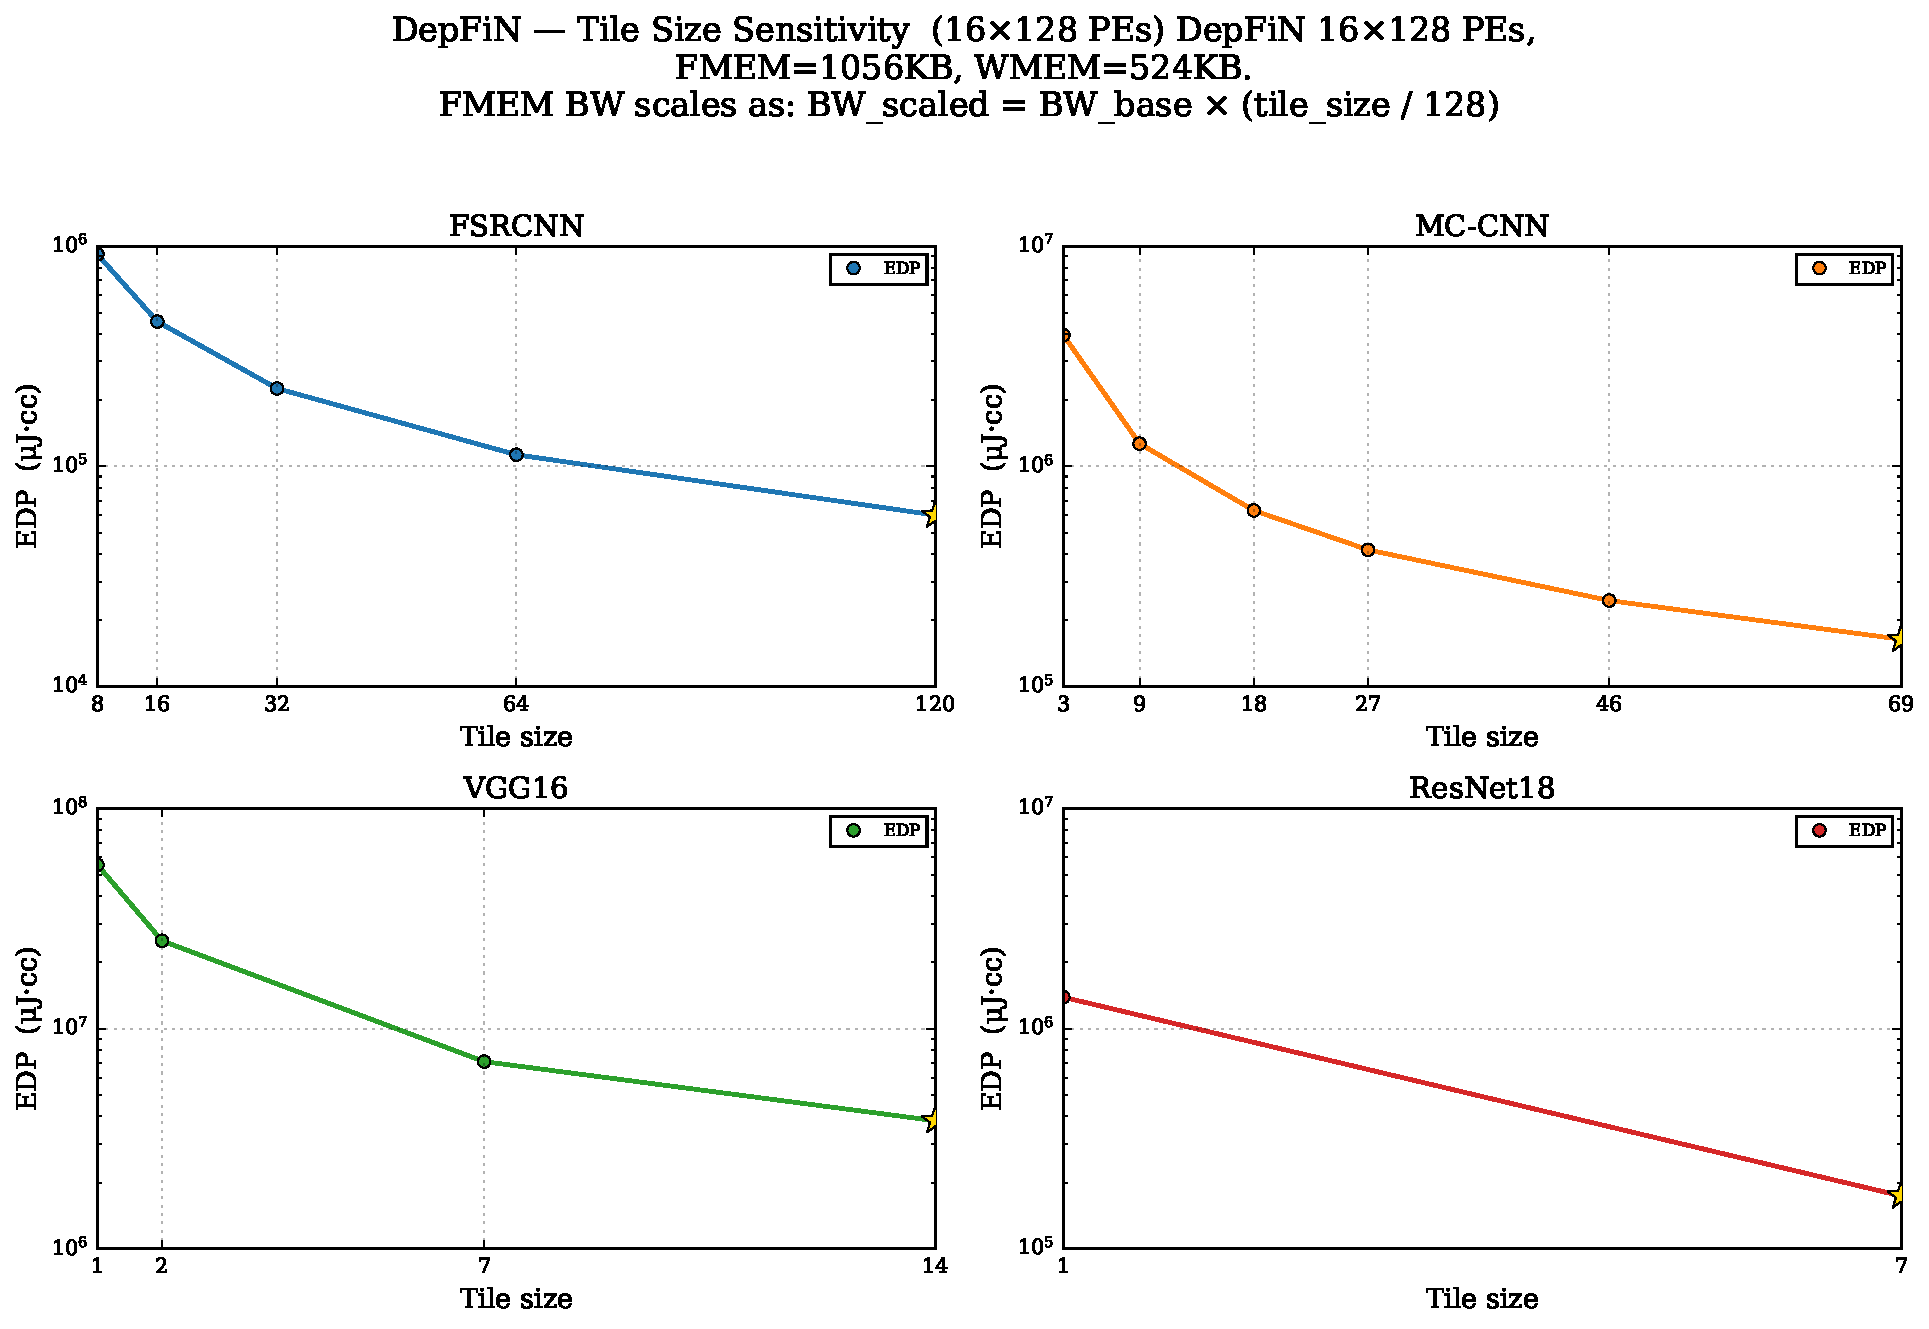
\includegraphics[width=0.85\textwidth]{plots/depfin_cs1_tile_sweep.pdf}
  \caption{DepFiN CS1: EDP vs\ tile size for each workload
    The gold star marks the best (minimum-EDP) tile.}
  \label{fig:depfin-cs1}
\end{figure}

\paragraph{FSRCNN (activation-dominant, no stride).}
As a representative example, FSRCNN is swept from an output tile width of 120
(93.8\,\% PE utilization) down to tile width of 8 (6.2\,\%).
The EDP degrades by $\approx 15\times$ driven
almost entirely by latency, which increases by $15\times$.
Energy, in contrast, rises by only $+4$\,\%.
The mild energy increase is explained by the weight re-read mechanism:
with an output tile width of 120 the Weight Memory is read $8.1 \times 10^{7}$~times,
whereas at output tile width of 8 the same weights are re-fetched
$1.2 \times 10^{9}$~times ($15\times$ more), because each of the
additional DRAM passes triggers a full reload of the weight set from Weight Memory.
DRAM reads and writes remain \emph{identical} across all tile sizes,
confirming that the degradation is internal to the on-chip hierarchy.

\paragraph{Weight-dominant workloads.}
VGG16 and ResNet18 exhibit a qualitatively similar trend, but with a
larger energy increase ($+25$\,\% and $+26$\,\% respectively from best
to worst tile), due to larger weight volumes to be reloaded.
The EDP degradation ranges from $8\times$ (ResNet18, tiles 7\,$\to$\,1)
to $15\times$ (VGG16, tiles 14\,$\to$\,1).

\paragraph{Considerations.}

For all four workloads, the largest feasible tile size minimizes EDP in DepFiN.
The dominant effect is latency: smaller tiles force more temporal
iterations at the DRAM level.
The effect of Energy is secondary and grows mainly through increased weight re-reads in the Weight Memory, but this effect is more pronounced for
weight-dominant workloads.
% ============================================================
%  N.2.2  DepFiN CS2: PE Aspect Ratio Sweep
% ============================================================
\subsection{DepFiN: PE Aspect Ratio (CS2)}
\label{sec:cs4-aspect}

\subsubsection{Motivation}
CS2 address a complementary question with respect to the precedent case studies:
\emph{given a fixed total PE budget, how should the array be shaped,
i.e.\ how many rows versus columns, to minimize EDP?}
CS2 fix the total number of PEs at
2\,048 and varying only the aspect ratio, from the extremely
column-heavy configuration $2 \times 1\,024$ to the extremely
row-heavy configuration $1\,024 \times 2$.
Memory sizes and register capacities are held constant at the
per-workload values used throughout the DepFiN experiments.

Because rows map to output channels~$Z$ and columns map to tile
width~$Q$, shifting PEs from columns to rows simultaneously reduces
the highest tile size available and increases the $Z$-parallelism.
The tile size, in turn, is chosen for the experiment as the largest divisor
of~$Q$ that fits within the available columns.
A strongly column-heavy shape therefore wastes rows (few $Z$ channels
processed per pass, many re-reads of input activations from the
Feature Memory), while a strongly row-heavy shape wastes columns (tiny
tile, many DRAM-level passes, many weight re-reads from the Weight
Memory).

The EDP curve is thus expected to be U-shaped, with a minimum at the
aspect ratio that best balances the two effects.

\subsubsection{Results}

Figure~\ref{fig:depfin-cs4} shows EDP (log scale, primary axis) and
energy ($\mu$J, linear scale, secondary axis) as a function of aspect
ratio for each workload.
The gold star marks the EDP-optimal configuration.

\begin{figure}[htbp]
  \centering
  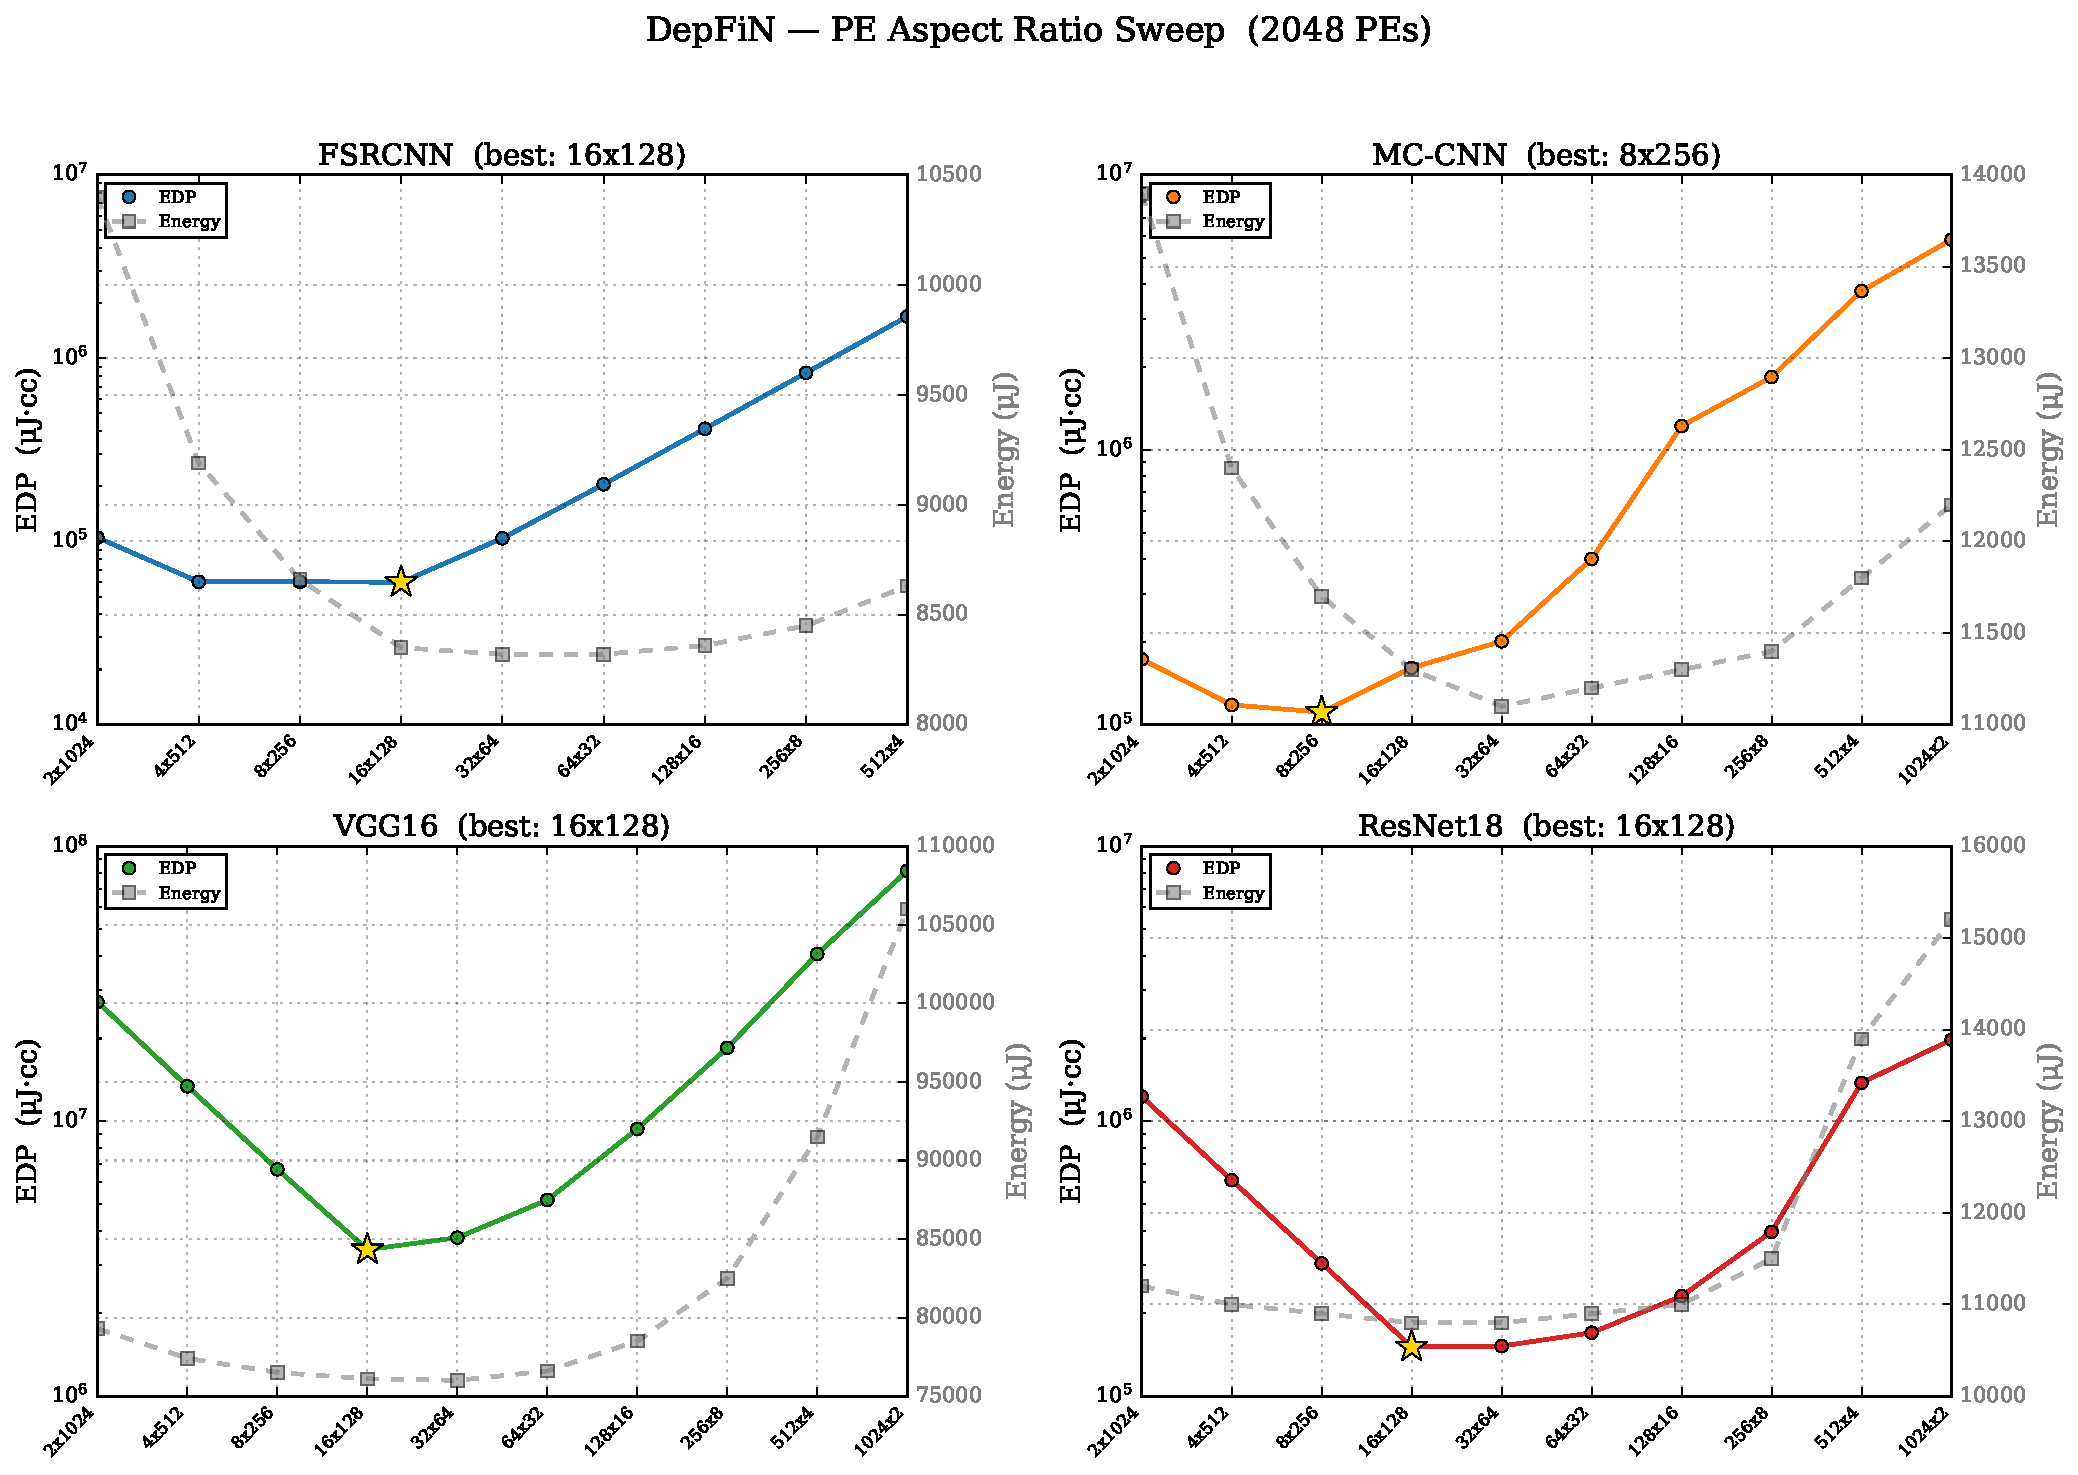
\includegraphics[width=0.9\textwidth]{plots/depfin_cs4_aspect_ratio.pdf}
  \caption{DepFiN CS2: EDP and energy vs.\ PE aspect ratio
    (total PEs\,=\,2\,048).
    The gold star marks the minimum-EDP configuration.}
  \label{fig:depfin-cs4}
\end{figure}

\paragraph{FSRCNN (activation-dominant).}
The EDP curve exhibits a broad minimum centered on $16 \times 128$, with the neighboring
configurations $4 \times 512$ and $8 \times 256$ within
5\,\% and 3\,\% respectively.
Moving toward the row-heavy end the EDP rises steeply: at $512 \times 4$, the increase is driven entirely by latency, which grows by $28\times$
from $16 \times 128$ configuration to $512 \times 4$, as the tile
shrinks and each additional DRAM pass reloads the full weight set.
Energy, in contrast, varies by only $\pm 20$\,\% across the entire
sweep, confirming that for activation-dominant workloads the dominant energy component, register-level operations, is largely insensitive to the
array shape.

\paragraph{MC-CNN (activation-dominant).}
MC-CNN is the only workload tried whose optimum shifts away from
$16 \times 128$ PE configuration: the best configuration is $8 \times 256$.
The shift occurs because MC-CNN's output spatial dimension
($Q = 1\,242$) benefit from the wider tile that 256
columns provide, reducing DRAM-level passes beyond what 128 columns
can achieve.
At the column-heavy extreme ($2 \times 1\,024$) the EDP is
$1.7\times$ worse, while at the row-heavy
extreme ($1\,024 \times 2$) it is
$53\times$ worse, making the U-shape strongly
asymmetric: the penalty for too many rows far exceeds the penalty for
too many columns.

\paragraph{Weight-dominant workloads (VGG16, ResNet18).}
Both workloads are optimized at $16 \times 128$.
VGG16 EDP drops sharply from $2 \times 1\,024$ to $16 \times 128$ with an $8\times$ improvement, then rises again at $1\,024 \times 2$ configuration, $24\times$ worse than the optimum.

The left-hand descent is driven by latency: at $2 \times 1\,024$ only
two output channels are mapped per pass, requiring many temporal
iterations over~$Z$, while at $16 \times 128$ the bottleneck layer's
channel count (64) is covered in four passes.
The right-hand ascent is driven by both latency and energy: as columns
shrink below 128 the tile fragments, weight memory re-reads multiply, and
energy increases by $+42$\,\%.
ResNet18 mirrors this pattern, with the EDP at the row-heavy extreme
$13\times$ above the optimum.

\paragraph{Considerations.}
All four workloads produce a U-shaped EDP curve, confirming that both
extremes of the aspect ratio are not suitable for these workloads.
The optimum lies near $16 \times 128$ for three of the four workloads
and at $8 \times 256$ for MC-CNN, whose large output spatial dimension
rewards a wider tile.
The curve is consistently asymmetric: but the rapidity of growing of EDP is determined by the activation or weight dominance of the workload.

% ============================================================
%  N.2.4  Eyeriss CS1: Weight Register Sizing
% ============================================================
\subsection{Eyeriss: Weight Register Sizing (CS1)}
\label{sec:eyeriss-cs1}

\subsubsection{Motivation}

In the Eyeriss-Like architecture every PE stores its assigned weight
filters in a local Weight Register (WReg).
When multiple layers are fused, a single PE must hold the weight
residuals for \emph{all} fused layers simultaneously, that is, the weight iterations
that are not spatially absorbed by the Systolic Array Rows (SARows) mapping.
The WReg is therefore the largest per-PE register in case of Weight-Dominant workloads, and it acts as the binding constraint on feasibility: if the required
weight footprint exceeds the WReg capacity, no valid mapping exists
for that PE configuration.

The trade-off between WReg size and the minimum number
of PEs can be expressed as:
%
\begin{itemize}
  \item A higher total PE count means that more weight factors are spatially absorbed, enabling a \emph{smaller} WReg.
  \item A smaller total PE count means that each PE must store more residual in its WReg, so it must to be \emph{larger}, at the cost of having higher energy access cost.
\end{itemize}

This case study answers to the question: \emph{what is the minimum weight register size that makes the
fused mapping feasible at this given PE count?}

CS1 answers this question by sweeping the WReg size at a given PE configuration ($\text{rows} \times \text{cols}$, up
to 16\,384 total PEs), in order to find the minimum WReg size feasible and the resulting energy and EDP.

The GlobalBuffer (128\,KB), input register, intermediate register, and
output register are held constant throughout.

\subsubsection{Results}

\paragraph{Weight-dominant workloads (VGG16, ResNet18).}

Table~\ref{tab:eyeriss-cs1-wreg} reports the minimum WReg size
required at three PE budgets, together with the configuration chosen
by the mapper and the resulting energy, latency, and EDP.

\begin{table}[htbp]
  \centering
  \caption{Eyeriss CS1: Minimum WReg size for a given PE budget
    (VGG16 and ResNet18, full fusion).
    For each row the PE budget is fixed and the smallest feasible WReg
    is reported.}
  \label{tab:eyeriss-cs1-wreg}
  \begin{tabular}{llrrrrr}
    \toprule
    Workload & PE budget & Min WReg & Config & Energy ($\mu$J) &
      Latency (cc) & EDP (J$\cdot$cc) \\
    \midrule
    VGG16    & 16\,384 & 1\,200  & $256 \times 64$  & $1.62 \times 10^{5}$
             & $5.46 \times 10^{6}$ & $9.04 \times 10^{5}$ \\
    VGG16    & 8\,192  & 2\,400  & $128 \times 64$  & $2.47 \times 10^{5}$
             & $5.68 \times 10^{6}$ & $1.42 \times 10^{6}$ \\
    VGG16    & 4\,096  & 4\,800  & $128 \times 32$  & $4.18 \times 10^{5}$
             & $6.72 \times 10^{6}$ & $2.82 \times 10^{6}$ \\
    \midrule
    ResNet18 & 16\,384 & 902     & $256 \times 64$  & $2.35 \times 10^{4}$
             & $3.04 \times 10^{6}$ & $7.36 \times 10^{4}$ \\
    ResNet18 & 8\,192  & 1\,800  & $128 \times 64$  & $3.28 \times 10^{4}$
             & $3.04 \times 10^{6}$ & $1.02 \times 10^{5}$ \\
    ResNet18 & 4\,096  & 3\,600  & $128 \times 32$  & $5.18 \times 10^{4}$
             & $3.06 \times 10^{6}$ & $1.60 \times 10^{5}$ \\
    \bottomrule
  \end{tabular}
\end{table}

The table reveals a regular scaling law.
For ResNet18 a designer with a 16\,384-PE budget needs at least
WReg\,=\,902 bytes, and only two PE configurations out of the entire
grid are feasible at that size.
Halving the PE budget to 8\,192 doubles the required register to
WReg\,=\,1\,800, and halving again to 4\,096 doubles it once more to
WReg\,=\,3\,600.

As stated, fewer spatial rows leave more weight
factors unabsorbed, and those residuals must be stored temporally in
the register.

VGG16 obeys the same doubling rule (1\,200 $\to$ 2\,400 $\to$ 4\,800)
at proportionally larger WReg values, reflecting its wider channels.

The energy consequence is substantial.
For ResNet18, moving from the 16\,384-PE point
 to the 4\,096-PE point
 increases energy by $2.2\times$,
because each weight access now touches a register that is $4\times$
larger.
Latency, however, stays nearly constant
(less than 1\% of difference), which indicates that the
computation is not memory-bound (\ref{sec:ps-latency}) once a feasible mapping exists.
The EDP therefore tracks energy closely, growing by $2.2\times$ over
the same range.

VGG16 shows both a steeper energy increase ($2.6\times$) and a moderate latency penalty ($\approx 23\,\%$), compounding into a $3.1\times$ EDP rise across the PE budget sweep. The latency degradation is driven by the middle layers (L2--L6, $Z{=}128$--$256$, $56{\times}56$--$112{\times}112$), where the constrained PE count increases weight traffic beyond the DRAM bandwidth capacity, causing memory stalls.



Figure~\ref{fig:eyeriss-cs1-inv} The horizontal axis is the PE budget and
the vertical axis is the minimum WReg required.
Reading the curve from left to right, one can directly read off the
register size that a given area constraint demands.

\begin{figure}[htbp]
  \centering
  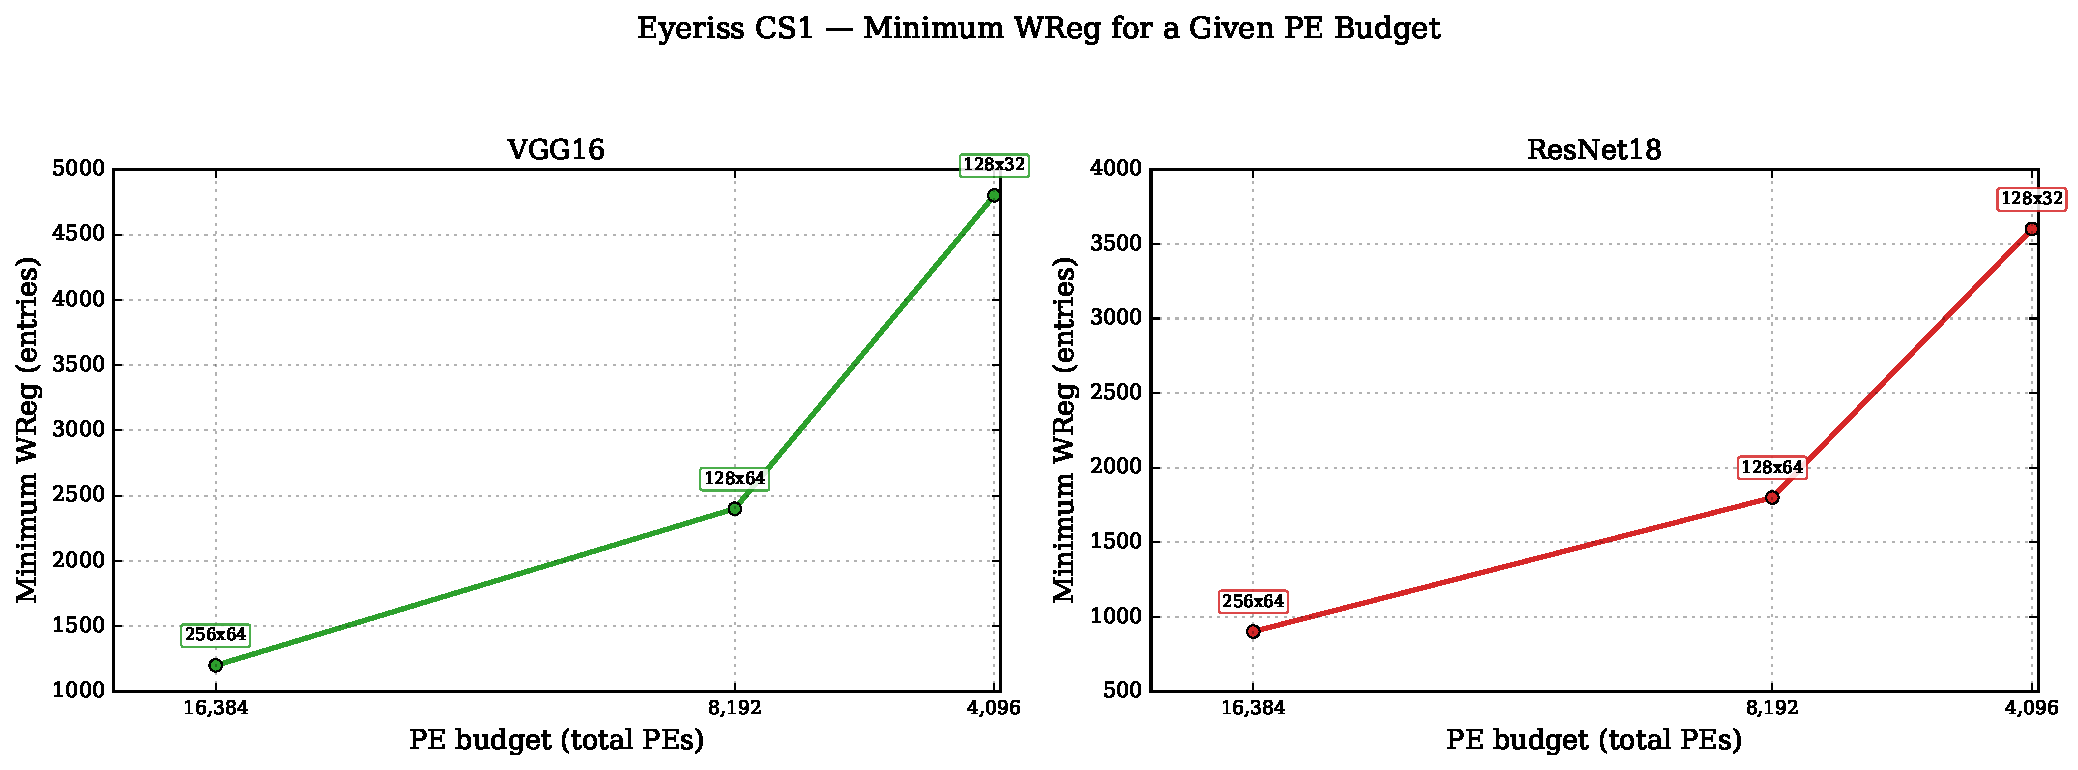
\includegraphics[width=0.85\textwidth]{plots/eyeriss_cs1_wreg_inverted.pdf}
  \caption{Eyeriss CS1: Minimum WReg required as a function of PE
    budget (VGG16 and ResNet18).}
  \label{fig:eyeriss-cs1-inv}
\end{figure}

\paragraph{Activation-dominant workloads (FSRCNN, MC-CNN).}
For these workloads the weight register is not the binding constraint.
FSRCNN and MC-CNN reaches feasibility for 1024 PEs at values of WReg lower than the value of default single layer
Eyeriss (384 bits).

Energy still scales linearly with register size, but the effect is
modest because the register is small in absolute terms.


\paragraph{Considerations.}
The weight register is a critical sizing knob for the Eyeriss-Like
architecture under full fusion.
For weight-dominant workloads, halving the PE budget roughly doubles
the required WReg, and the larger register inflates energy in
proportion, because every weight read access a physically larger SRAM
structure.
At the number of PEs tried, latency is less affected, so EDP tracks energy mainly.
For activation-dominant workloads the register is non-binding and can
be kept small without limiting feasibility.
% ============================================================
%  N.2.5  Eyeriss CS2 & CS3: Activation Register Sizing
% ============================================================
\subsection{Eyeriss: Activation Register Sizing (CS2, CS3)}
\label{sec:eyeriss-cs2-cs3}

\subsubsection{Motivation}

Besides the weight register examined in CS1, every PE in the
Eyeriss-Like architecture contains three local storage
structures: an \emph{input register} (InReg), which buffers the
first layer's input activations; an \emph{intermediate register}
(IntReg), which buffers the activation values exchanged between
consecutive fused layers; and an \emph{output register} (OutReg),
which holds the final-layer output before it is written back to the
GlobalBuffer.

Of these three, only IntReg (CS2) is genuinely affected by fusion.
The InReg sees exclusively the network's input, regardless of how
many layers are fused: intermediate activations produced inside the
fusion chain never pass through InReg, they are routed to IntReg
instead.
Similarly, the OutReg stores only the last fused layer's output
channel residual, so its footprint does not grow with the number of
fused layers.

We will analyze InReg and OutReg in a unique case study CS3.

Under full fusion the IntReg must accommodate the residual channel
factors of \emph{all} intermediate activations, i.e.\ the $Z_i$
values that the systolic array columns (SACols) cannot absorb.
The footprint therefore scales with the number of fused layers and
with the width of their channel dimensions.


% ────────────────────────────────────────────────────────────────────
\label{sec:eyeriss-cs2}

\paragraph{CS2 per Weight-dominant workloads (ResNet18, VGG16)}: \\



The table reveals the same doubling rule observed for WReg in CS1.


Figure~\ref{fig:eyeriss-cs2-inv} the horizontal axis is the PE budget and the vertical axis is
the minimum IntReg that makes the fused mapping feasible.
Reading the curve from left to right, one can directly read off the
register size that a given area constraint demands.
The slope is consistent with the doubling rule: every $2\times$
reduction in PE budget roughly doubles the minimum IntReg.

\begin{figure}[htbp]
  \centering
  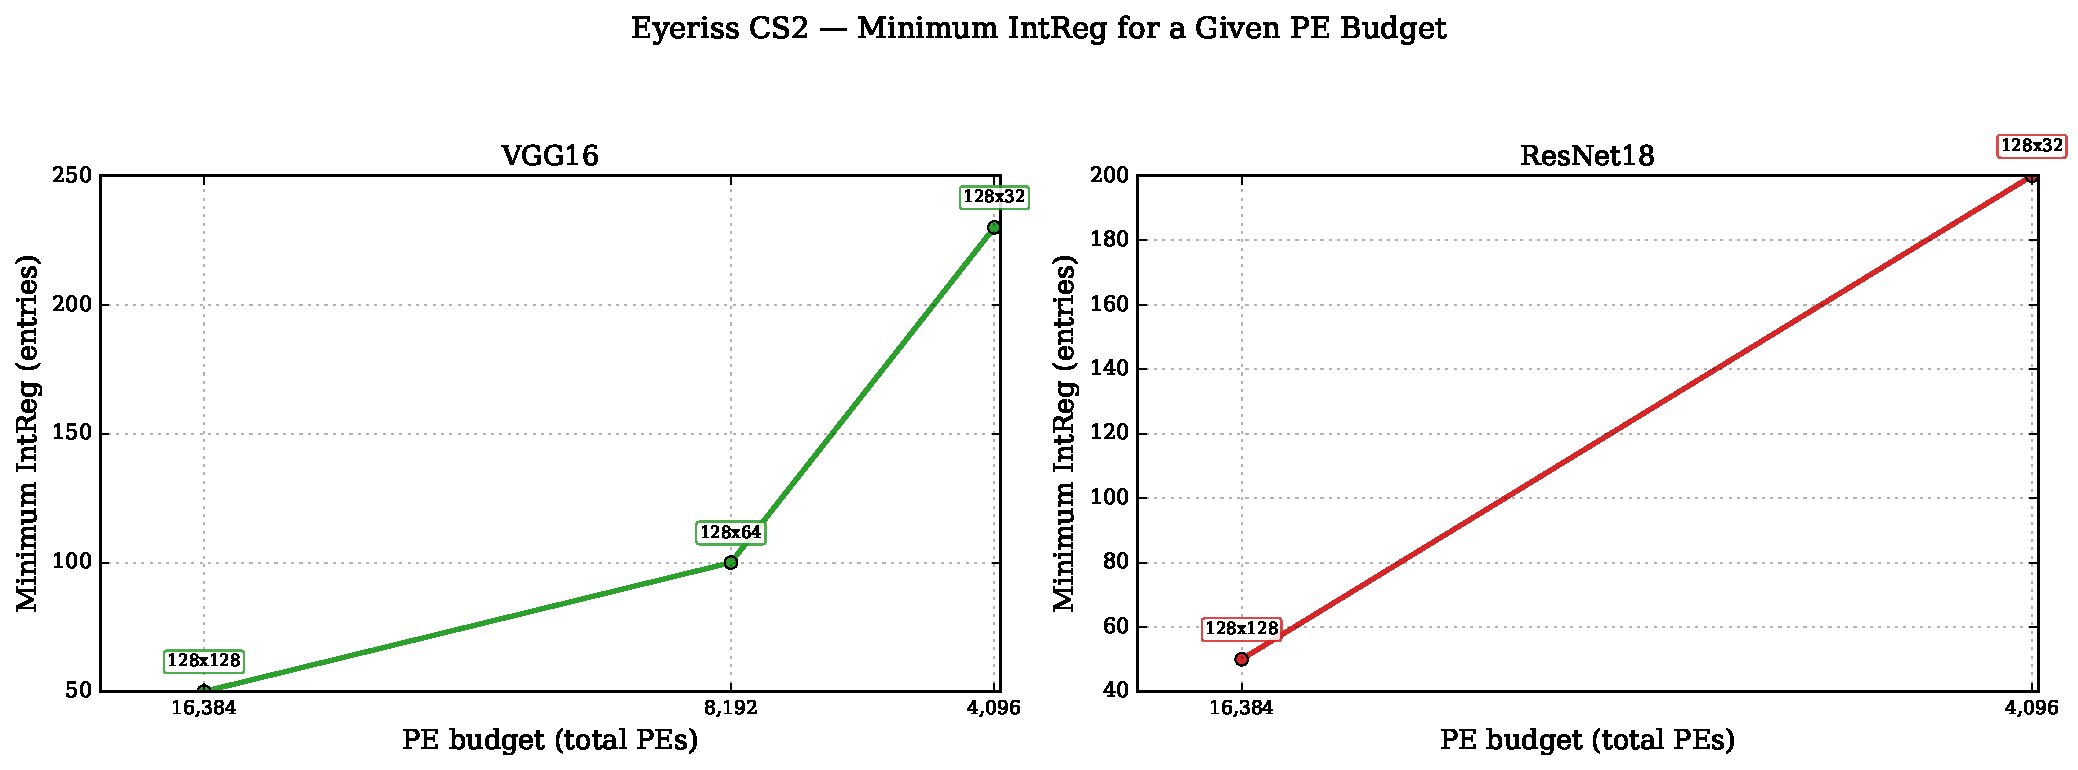
\includegraphics[width=0.85\textwidth]{plots/eyeriss_cs2_intreg_inverted.pdf}
  \caption{Eyeriss CS2: Minimum IntReg required as a function of PE
    budget (VGG16 and ResNet18, full fusion).}
  \label{fig:eyeriss-cs2-inv}
\end{figure}
Figure~\ref{fig:eyeriss-cs2-inv} (top row) reports the energy consumption at the minimum-PE configuration for each IntReg size. Energy grows monotonically with IntReg capacity, as a larger register incurs a higher per-read access cost. For ResNet18, the energy increases by $1.4\times$ when scaling from IntReg\,=\,50 to IntReg\,=\,1\,000. This is a relatively modest penalty compared to the $2.2\times$ energy span caused by the WReg expansion in CS1, a difference that directly reflects the weight-dominant nature of the workload.


\paragraph{CS2 per Activation-dominant workloads (FSRCNN, MC-CNN).}
For these workloads the intermediate register is not a binding
constraint.
In both cases, even with a budget of PEs of 1024, the intermediate footprint is small (16) because these
networks have few fused layers and narrow channels.

% ────────────────────────────────────────────────────────────────────
\label{sec:eyeriss-cs3}

\paragraph{CS3}
The output register stores only the last fused layer's channel
residual, so its footprint is inherently smaller than that of IntReg
or WReg.
The original single-layer Eyeriss design uses OutReg with a capacity of 16 bytes,
and this value turns out to be sufficient for full fusion as well at
the PE budgets that WReg and IntReg already demand.

The curves lie well below the corresponding CS1 and CS2 curves at
every PE budget, confirming that OutReg is the least binding of the
three register types.
For activation-dominant workloads (FSRCNN, MC-CNN) the output register
has no effect on the PE count whatsoever: all tested PEs budget have could support the OutReg size of the Eyeriss single layer configuration.

\begin{figure}[htbp]
  \centering
  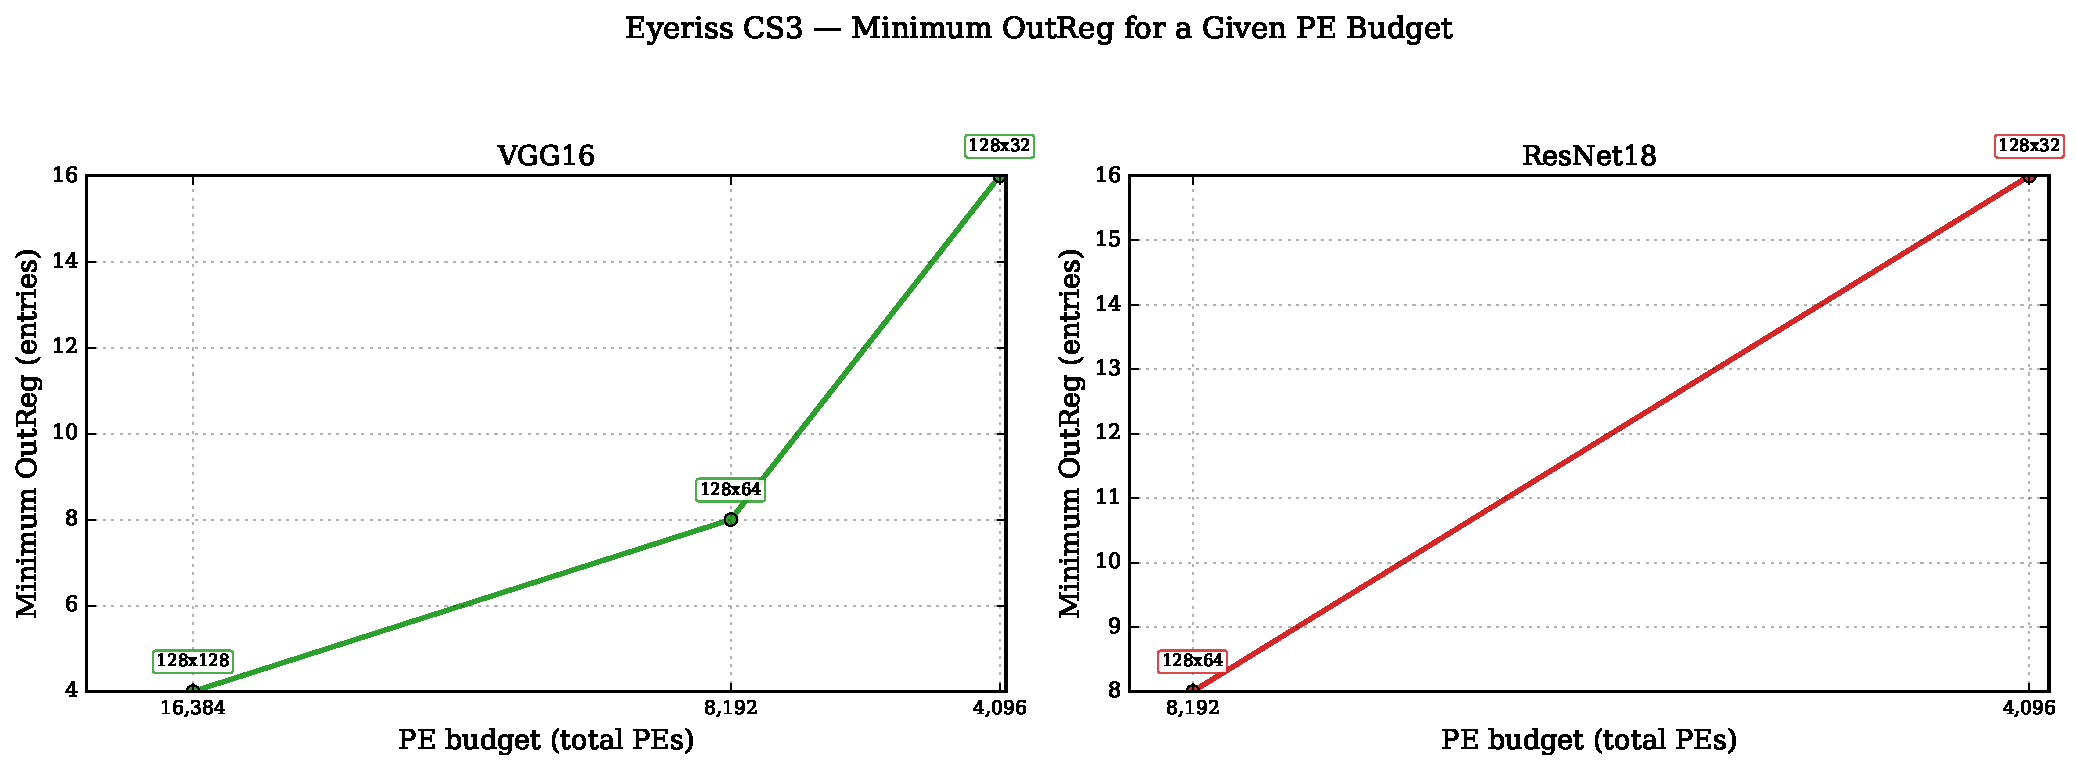
\includegraphics[width=0.85\textwidth]{plots/eyeriss_cs3_outreg_inverted.pdf}
  \caption{Eyeriss CS3: Minimum OutReg required as a function of PE
    budget (VGG16 and ResNet18, full fusion).}
  \label{fig:eyeriss-cs3-inv}
\end{figure}

Analogous reasoning can be applied for Input register sizing.


\paragraph{Considerations}
The intermediate register follows the same PE-doubling-per-halving
rule as the weight register, but its absolute footprint is roughly
one order of magnitude smaller, so it becomes binding only at PE
counts well below the WReg minimum.
The output register is even less constraining: with OutReg with a capacity 16 bytes
(the value used in the original single-layer Eyeriss), the fused
mapping is already feasible at the PE budgets imposed by WReg.
The input register is unaffected by fusion too, because it
handles only the first layer's input and its footprint remains the
same as in single-layer execution.
% ============================================================
%  N.2.5  Eyeriss CS5: PE Array Aspect Ratio
% ============================================================
\subsection{Eyeriss: PE Array Aspect Ratio (CS5)}
\label{sec:eyeriss-cs5}

\subsubsection{Motivation}
Optimizing the PE array aspect ratio for EDP  (see Section \ref{sec:cs4-aspect}) is also essential in Eyeriss, because its spatial mapping distributes different loop dimensions across the two axes. Rows absorb weight-related factors ($C$, $S$, $Z$), whereas columns absorb output channel factors. 

Therefore, a row-heavy array absorbs more weight factors spatially but forces larger channel residuals in the column direction, while a column-heavy configuration exhibits the inverse behavior. Ultimately, the optimal shape is governed by the relative size of the weight and activation dimensions in the fused workload.

To evaluate this trade-off, CS5 sweeps all power-of-two factorizations of a fixed PE budget (2,048 PEs for FSRCNN and MC-CNN; 16,384 PEs for VGG16 and ResNet18), tracking the resulting energy, latency, and EDP for every feasible mapping. 


\subsubsection{Results}

\paragraph{ResNet18 (16\,384 PEs).}
Table~\ref{tab:eyeriss-cs5} lists the feasible configurations for
ResNet18, with a weight register size fixed.
Seven aspect ratios are feasible, from
$256 \times 64$ to the extreme row-heavy $16{,}384 \times 1$.
Latency is constant across all configurations, therefore the EDP ranking is determined entirely
by energy.
The best configuration is $256 \times 64$, and energy increases gently as
the array becomes more row-heavy.

The total variation is only $2.6\%$, indicating that for ResNet18 the
aspect ratio has a negligible impact once feasibility is achieved.

\begin{table}[htbp]
  \centering
  \caption{Eyeriss CS5: PE aspect ratio sweep for ResNet18
    (16\,384 total PEs, full fusion).
    Best EDP marked with~$\star$.}
  \label{tab:eyeriss-cs5}
  \begin{tabular}{lrrrr}
    \toprule
    Config & Rows & Cols & Energy ($\mu$J) & EDP (J$\cdot$cc) \\
    \midrule
    $256 \times 64$\,$\star$
           & 256   & 64  & $2.35 \times 10^{4}$ & $7.36 \times 10^{4}$ \\
    $512 \times 32$
           & 512   & 32  & $2.37 \times 10^{4}$ & $7.37 \times 10^{4}$ \\
    $1024 \times 16$
           & 1024  & 16  & $2.40 \times 10^{4}$ & $7.46 \times 10^{4}$ \\
    $2048 \times 8$
           & 2048  &  8  & $2.41 \times 10^{4}$ & $7.50 \times 10^{4}$ \\
    $4096 \times 4$
           & 4096  &  4  & $2.41 \times 10^{4}$ & $7.50 \times 10^{4}$ \\
    $8192 \times 2$
           & 8192  &  2  & $2.41 \times 10^{4}$ & $7.50 \times 10^{4}$ \\
    $16384 \times 1$
           &16384  &  1  & $2.41 \times 10^{4}$ & $7.50 \times 10^{4}$ \\
    \bottomrule
  \end{tabular}
\end{table}
The underlying reason is that ResNet18 features deep channel dimensions ($Z$ up to 512) that easily saturate a moderate column count. At 64~columns, the spatial mapping mechanism (\texttt{SACols}) effectively absorbs the most $Z$ factors. Conversely, if the array is constrained to fewer than 64~columns, the mapper is forced to handle the excess $Z$ dimensions temporally. This temporal folding increases the required capacity of the weight register to accommodate the larger residuals, which marginally raises the energy cost per access.

\paragraph{VGG16 (16\,384 PEs).}
Seven power-of-two factorizations from $256 \times 64$ to
$16{,}384 \times 1$ are feasible, all sharing the same latency.
The best EDP is $512 \times 32$, tied with $256 \times 64$.
Energy rises by $4.1\%$ at
$2{,}048 \times 8$ and plateaus thereafter, mirroring the ResNet18
behavior.

\paragraph{FSRCNN (2\,048 PEs).}
FSRCNN exhibits a broader feasibility range, with nine
power-of-two factorizations from $8 \times 256$ to $2{,}048 \times 1$
being feasible.
The best EDP is the most column-heavy configuration,
$8 \times 256$.
Energy is $5.7\%$ lower at $8 \times 256$ than at $64 \times 32$ and
beyond, where it plateaus.


\paragraph{MC-CNN (2\,048 PEs).}
Nine configurations are feasible from $8 \times 256$ to $2{,}048 \times 1$.
The best EDP is $128 \times 16$, tying with $256 \times 8$ through
$2{,}048 \times 1$, while $16 \times 128$ is within $0.2\%$
and offers the lowest latency among competitive configurations.
The most column-heavy configuration ($8 \times 256$) has higher latency because only 8 rows cannot absorb enough
weight factors spatially, forcing more temporal iterations.
MC-CNN therefore favors a moderate aspect ratio that balances row
absorption of weights with column distribution of channels.


\paragraph{Cross-workload comparison.}
Figure~\ref{fig:eyeriss-cs5} presents the energy (top row) and EDP
(bottom row) for all four workloads.
Two patterns emerge.
First, the weight-dominant workloads (VGG16, ResNet18) show nearly
flat energy and EDP curves across all seven feasible aspect ratios,
with total variation below $4.1\%$ for VGG16 and $2.6\%$ for
ResNet18.
Second, the activation-dominant workloads (FSRCNN, MC-CNN) display
a mild preference for column-heavy configurations, where the Systolic Array Columns (SACols)
mechanism can distribute channel factors more effectively.
In all cases the EDP variation across feasible aspect ratios is
modest ($< 6\%$ for FSRCNN, $< 4.1\%$ for VGG16).

\begin{figure}[htbp]
  \centering
  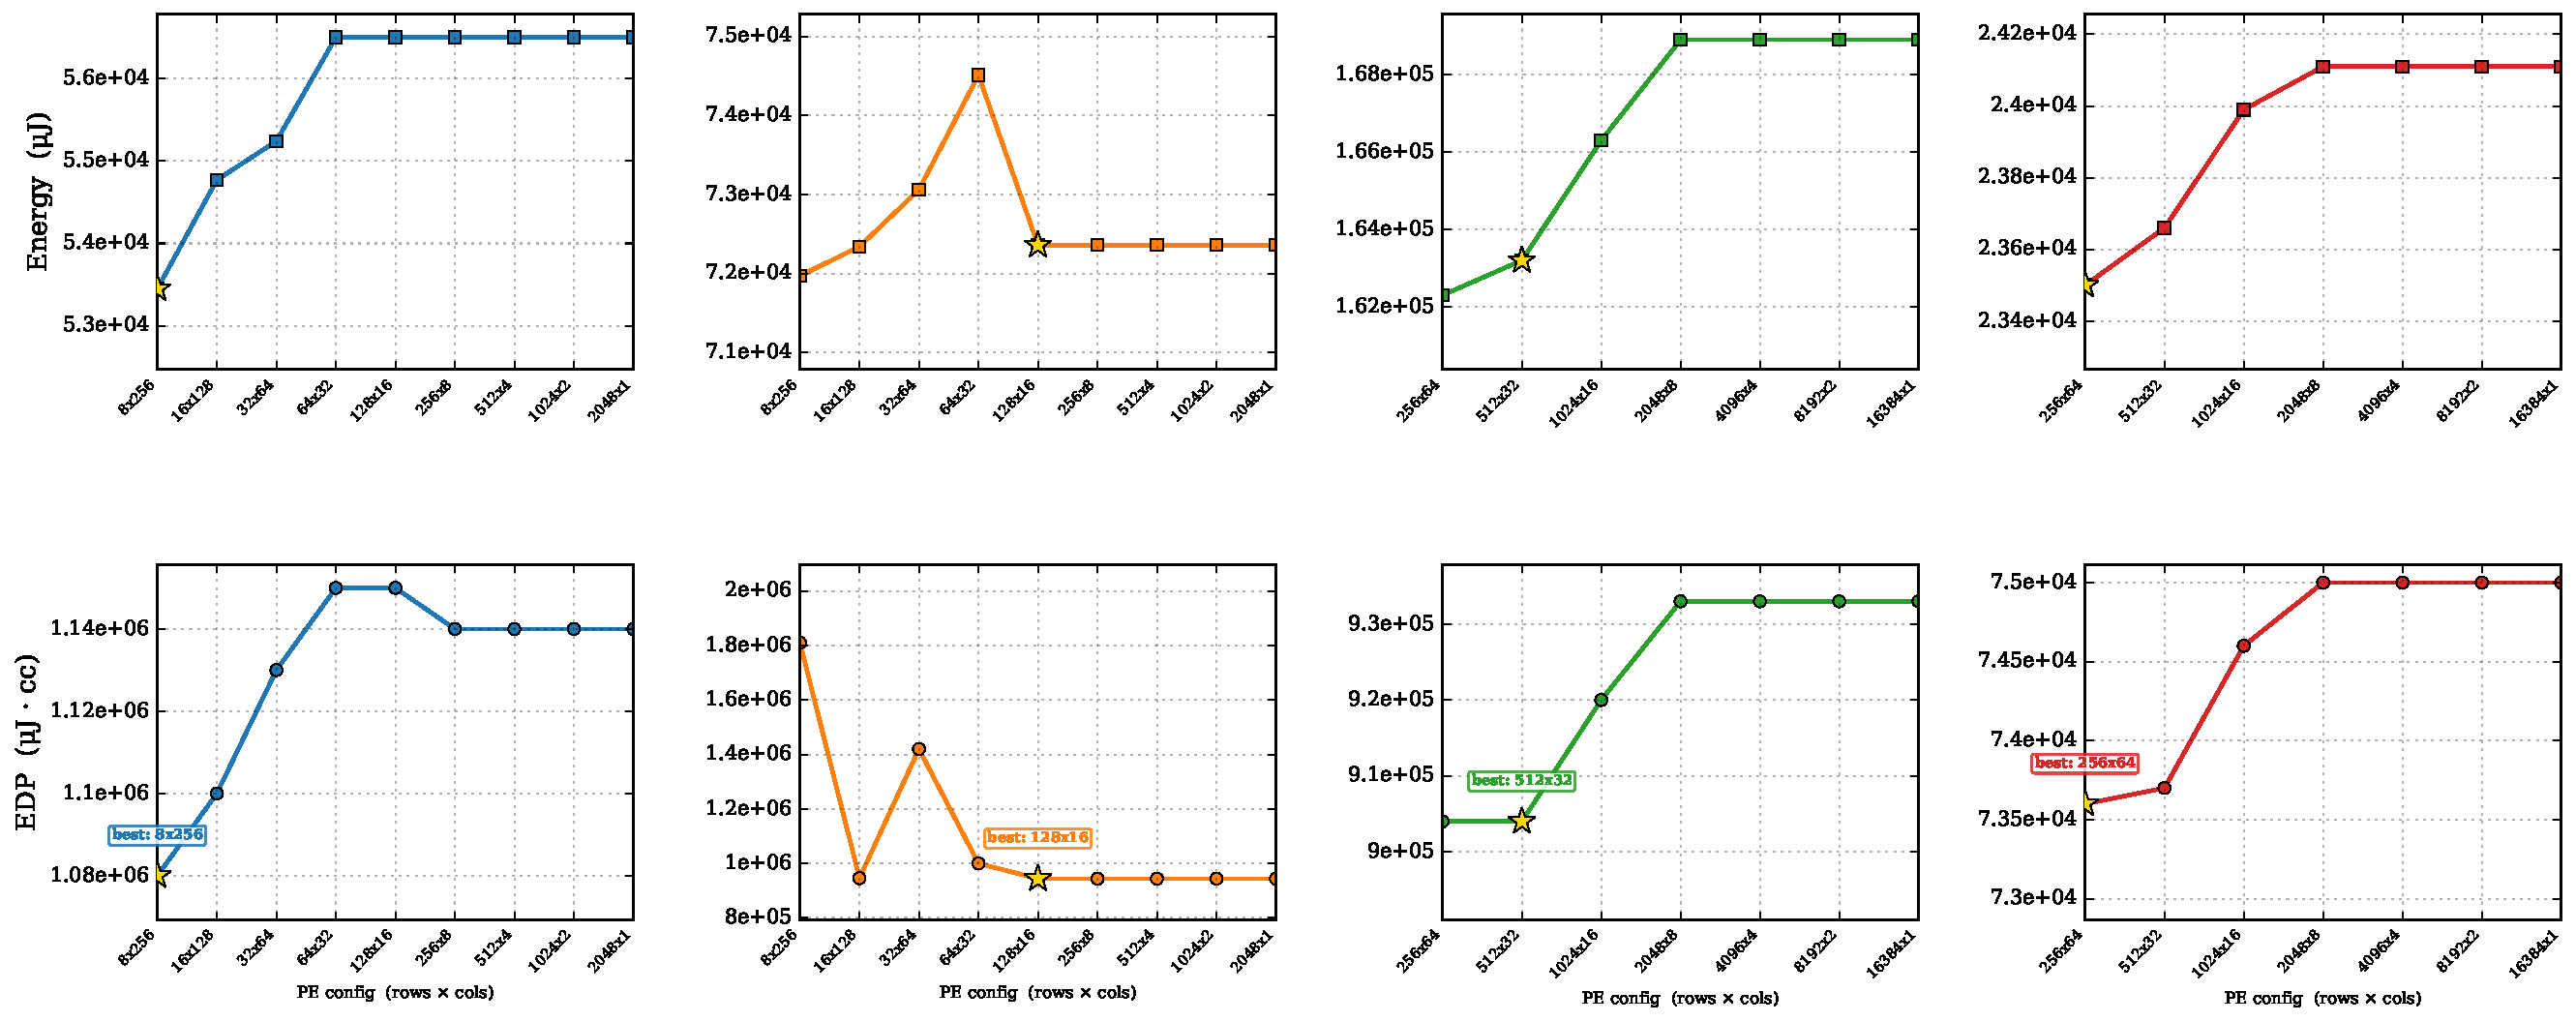
\includegraphics[width=0.95\textwidth]{plots/eyeriss_cs5_aspect_ratio.pdf}
  \caption{Eyeriss CS5: Energy (top) and EDP (bottom) vs.\ PE aspect
    ratio at fixed total PEs.
    Stars mark the best-EDP configuration for each workload.}
  \label{fig:eyeriss-cs5}
\end{figure}

\paragraph{Considerations}
Once the register sizes are set to satisfy the fused mapping
constraints, the PE aspect ratio has limited influence on energy and
EDP.
Column-heavy configurations offer a small advantage for workloads with
narrow channels, while weight-dominant workloads show nearly flat
curves regardless of aspect ratio once registers are adequately sized.

\newpage

% ============================================================
%  N.3  Layer Fusion Analysis
% ============================================================
\section{Layer Fusion Analysis}
\label{sec:fusion}

This section evaluates the benefit of layer fusion by comparing
fused, partial fused and non-fused execution on the same hardware architecture.
Two scenarios are considered: Scenario~A sizes the architecture
for full fusion and runs all three modes (full, partial, single)
on it; Scenario~B sizes the architecture for partial fusion only,
removing the full-fusion configuration to test whether a smaller
design can still capture most of the fusion benefit.



% ============================================================
%  N.3.1  Full-Sized Architecture: Fusion Mode Comparison
% ============================================================
\subsection{Full-Sized Architecture: Fusion Mode Comparison (Scenario~A)}
\label{sec:fusion-full-sized}

\subsubsection{Motivation}

The case studies presented in Sections~\ref{sec:eyeriss-cs1}
through~\ref{sec:eyeriss-cs5} focused on how individual
architectural parameters, such as register sizes and PE aspect
ratios, interact with the fusion mapping.
This section shifts perspective and answers the question:
\emph{does layer fusion actually improve the end-to-end efficiency
of a DNN accelerator on the same architecture instance, and under what conditions?}

To answer this, we define three execution modes on the \textbf{same
architecture instance}, which is sized to support full fusion of the
entire workload (Scenario~A):
\begin{enumerate}
  \item \textbf{Full fusion.}
        All convolutional layers are fused into a single mapping.
        Intermediate activations are kept entirely on chip, reducing
        DRAM traffic to the network's input and final output only.
  \item \textbf{Partial fusion (sum).}
        Consecutive layer groups are fused independently.
        The total cost is the sum of all fused evaluations.
        DRAM traffic is reduced for each group, but intermediate
        activations between non-fused layers still traverse DRAM.
  \item \textbf{Single-layer (sum).}
        Each layer is mapped in isolation, and the total cost is
        the sum of all individual layer evaluations.
        Every intermediate activation is written to and read back
        from DRAM.
\end{enumerate}

The architecture used for each workload is the \textbf{same} full-fusion
configuration determined by the PE and memory sizing studies done
(Table~\ref{tab:fusion-auto-configs}).
Running partial and single-layer modes on a full-fusion-sized
architecture provides a fair comparison because all three modes
share identical hardware; only the inter-layer mapping
strategy differs.

\begin{table}[htbp]
  \centering
  \caption{Architecture configurations used for Scenario~A
    (full-fusion-sized).
    Memory sizes refer to the DepFiN feature-memory (fmem) and
    weight-memory (wmem), or the Eyeriss GlobalBuffer (GB) and
    per-PE weight register (WReg).}
  \label{tab:fusion-auto-configs}
  \begin{tabular}{ll rr rr}
    \toprule
    & & \multicolumn{2}{c}{DepFiN} & \multicolumn{2}{c}{Eyeriss} \\
    \cmidrule(lr){3-4} \cmidrule(lr){5-6}
    Workload & PEs
      & fmem & wmem
      & GB & WReg \\
    \midrule
    FSRCNN   & $16 \times 128$ / $128 \times 16$
      & 576\,KB  & 19\,KB
      & 128\,KB  & 384 \\
    MC-CNN   & $8 \times 256$\, / $256 \times 8$
      & 522\,KB  & 32\,KB
      & 128\,KB  & 384 \\
    VGG16    & $16 \times 128$ / $512 \times 32$
      & 568\,KB  & 14\,366\,KB
      & 128\,KB  & 1\,200 \\
    ResNet18 & $16 \times 128$ / $512 \times 32$
      & 266\,KB  & 10\,738\,KB
      & 128\,KB  & 902 \\
    \bottomrule
  \end{tabular}
\end{table}

The following analysis is organized around three metrics, each
normalized to the full-fusion value, and concludes with the
DRAM traffic reduction and a summary of the key findings.

\subsubsection{Results}

% ── Energy ──────────────────────────────────────────────────
\paragraph{Energy (Figure~\ref{fig:fusion-energy-norm}).}
Whether full fusion saves or wastes energy depends critically on
the balance between two opposing effects: the elimination of DRAM
traffic for intermediate activations and the increased per-access
cost of the enlarged on-chip memories required to support fusion.
At 160\,pJ\,/\,byte for DRAM
(Section~\ref{sec:energy-model}), the outcome is
workload-dependent and architecture-dependent.


On \textbf{DepFiN}, full fusion is the most energy-efficient mode
for the two activation-dominant workloads.
FSRCNN in single-layer mode consumes $4.38\times$ the full-fusion
energy, and MC-CNN consumes $1.73\times$.
The explanation is that these workloads generate massive
intermediate-activation volumes (Section~\ref{sec:dram-traffic}),
and the DRAM energy eliminated by fusion
vastly exceeds the extra on-chip cost (576\,KB for FSRCNN, 522\,KB for MC-CNN).
Partial fusion also benefits, sitting at $1.47\times$ full for
FSRCNN and $1.43\times$ for MC-CNN.

For the weight-dominant workloads on DepFiN, the picture reverses.
VGG16 single-layer execution costs only $7.4\%$ of the
full-fusion energy, and ResNet18 costs $17.3\%$.
Fusion requires a weight memory of 14\,366\,KB (VGG16) or
10\,738\,KB (ResNet18) to hold all weights on chip
simultaneously.
Every weight access through these large memories incurs an
elevated per-access energy that compounds across billions of multiply accumulations (MACs).
Because the intermediate-activation volume is comparatively small,
the DRAM savings are insufficient to compensate.
Partial fusion partially mitigates this: its normalized energy is
$0.49$ for VGG16 and $0.75$ for ResNet18, confirming that fusing
only a few layers at a time requires less inflated memory.

On \textbf{Eyeriss}, full fusion is roughly energy-neutral for
FSRCNN (single\,$= 0.985\times$\,full), suggesting that the DRAM
savings and the register overhead nearly cancel.
For all other workloads, full fusion is again the most expensive
mode: MC-CNN single costs $45.0\%$ of full, VGG16 single costs
$5.9\%$, and ResNet18 single costs $12.6\%$.
The Eyeriss energy penalty is driven by the replicated register
architecture: with 16\,384~PEs for VGG16, the aggregate weight
register capacity is $19.7$~million
bytes ($1{,}200 \times 16{,}384$), each contributing to per-access energy.
Despite the high DRAM cost, the vast volume of on-chip accesses
through these large registers dominates the energy budget.
Partial fusion is consistently cheaper than full fusion on
Eyeriss, with normalized values of $0.66$ (FSRCNN), $0.65$
(MC-CNN), $0.39$ (VGG16), and $0.69$ (ResNet18).

\begin{figure}[htbp]
  \centering
  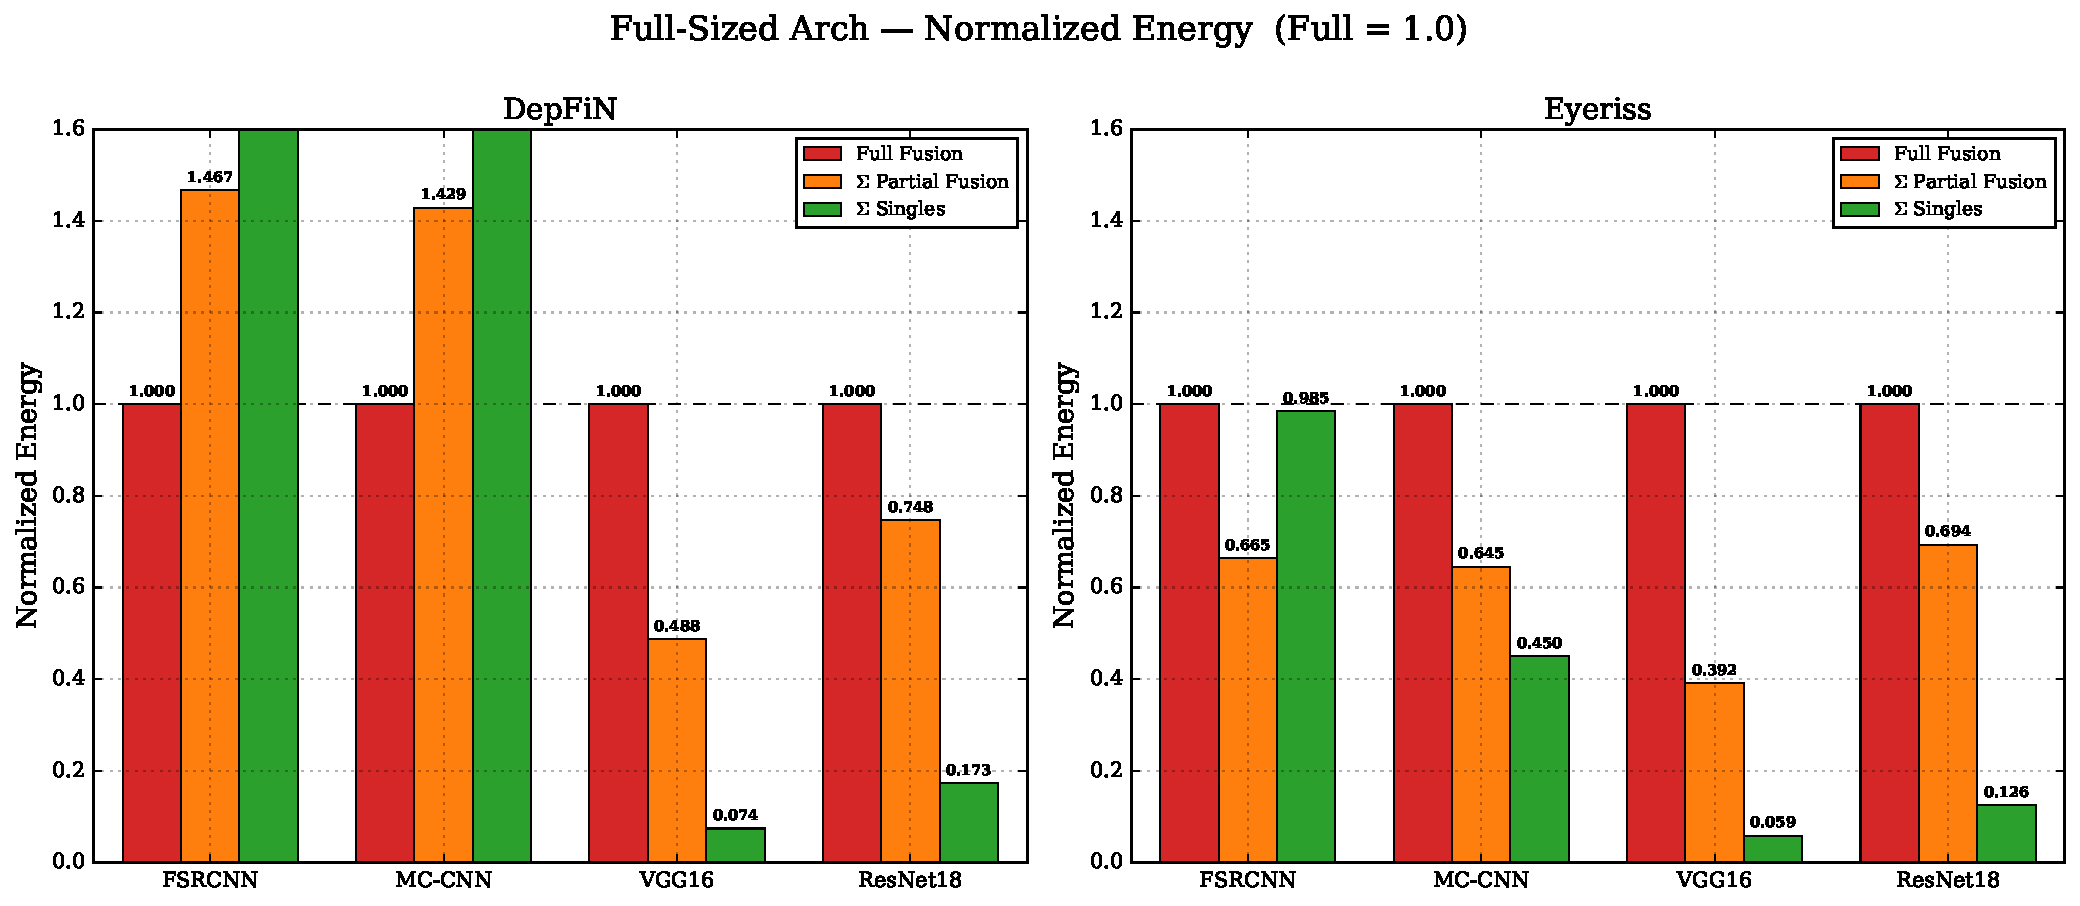
\includegraphics[width=0.95\textwidth]{plots/fusion_auto_energy_norm.pdf}
  \caption{Scenario~A: Normalized energy (Full~Fusion\,=\,1.0).
    Bars below 1.0 indicate lower energy than full fusion.
    Values annotated above each bar.}
  \label{fig:fusion-energy-norm}
\end{figure}



% ── Latency ─────────────────────────────────────────────────
\paragraph{Latency (Figure~\ref{fig:fusion-latency-norm}).}
Full fusion delivers latency benefits whose magnitude depends on the workload and architecture.

For the activation-dominant workloads, full fusion is clearly
faster on both architectures.
FSRCNN enjoys a $47.6\%$ latency saving on DepFiN and $45.6\%$
on Eyeriss, while MC-CNN saves $42.3\%$ on DepFiN and $15.7\%$
on Eyeriss (Figure~\ref{fig:fusion-latency-savings}).
These workloads have large intermediate-activation volumes
relative to their weight volumes, so eliminating the DRAM
round-trips for activations removes the dominant bottleneck from
the execution timeline.

For the weight-dominant workloads the behavior diverges across
architectures.
On Eyeriss, full fusion still reduces latency compared to the
single-layer sum: VGG16 saves $21.2\%$ and ResNet18 saves
$7.8\%$.
On DepFiN, however, full fusion is \emph{slower} than the
single-layer sum: VGG16 loses $11.3\%$ and ResNet18 loses
$30.3\%$.
Eyeriss avoids this penalty because its distributed per-PE
register architecture keeps each layer's weight factors local,
allowing to compute without a unique
shared memory contention point for all the layers, the weight memory.

Partial fusion tracks the full-fusion latency closely in most
cases: the ratio ranges from $0.87\times$ (ResNet18, DepFiN) to
$1.07\times$ (VGG16, Eyeriss), indicating that the latency
benefit of fusion is captured almost entirely by pairwise fusion,
with little additional gain from fusing all layers
simultaneously.

\begin{figure}[htbp]
  \centering
  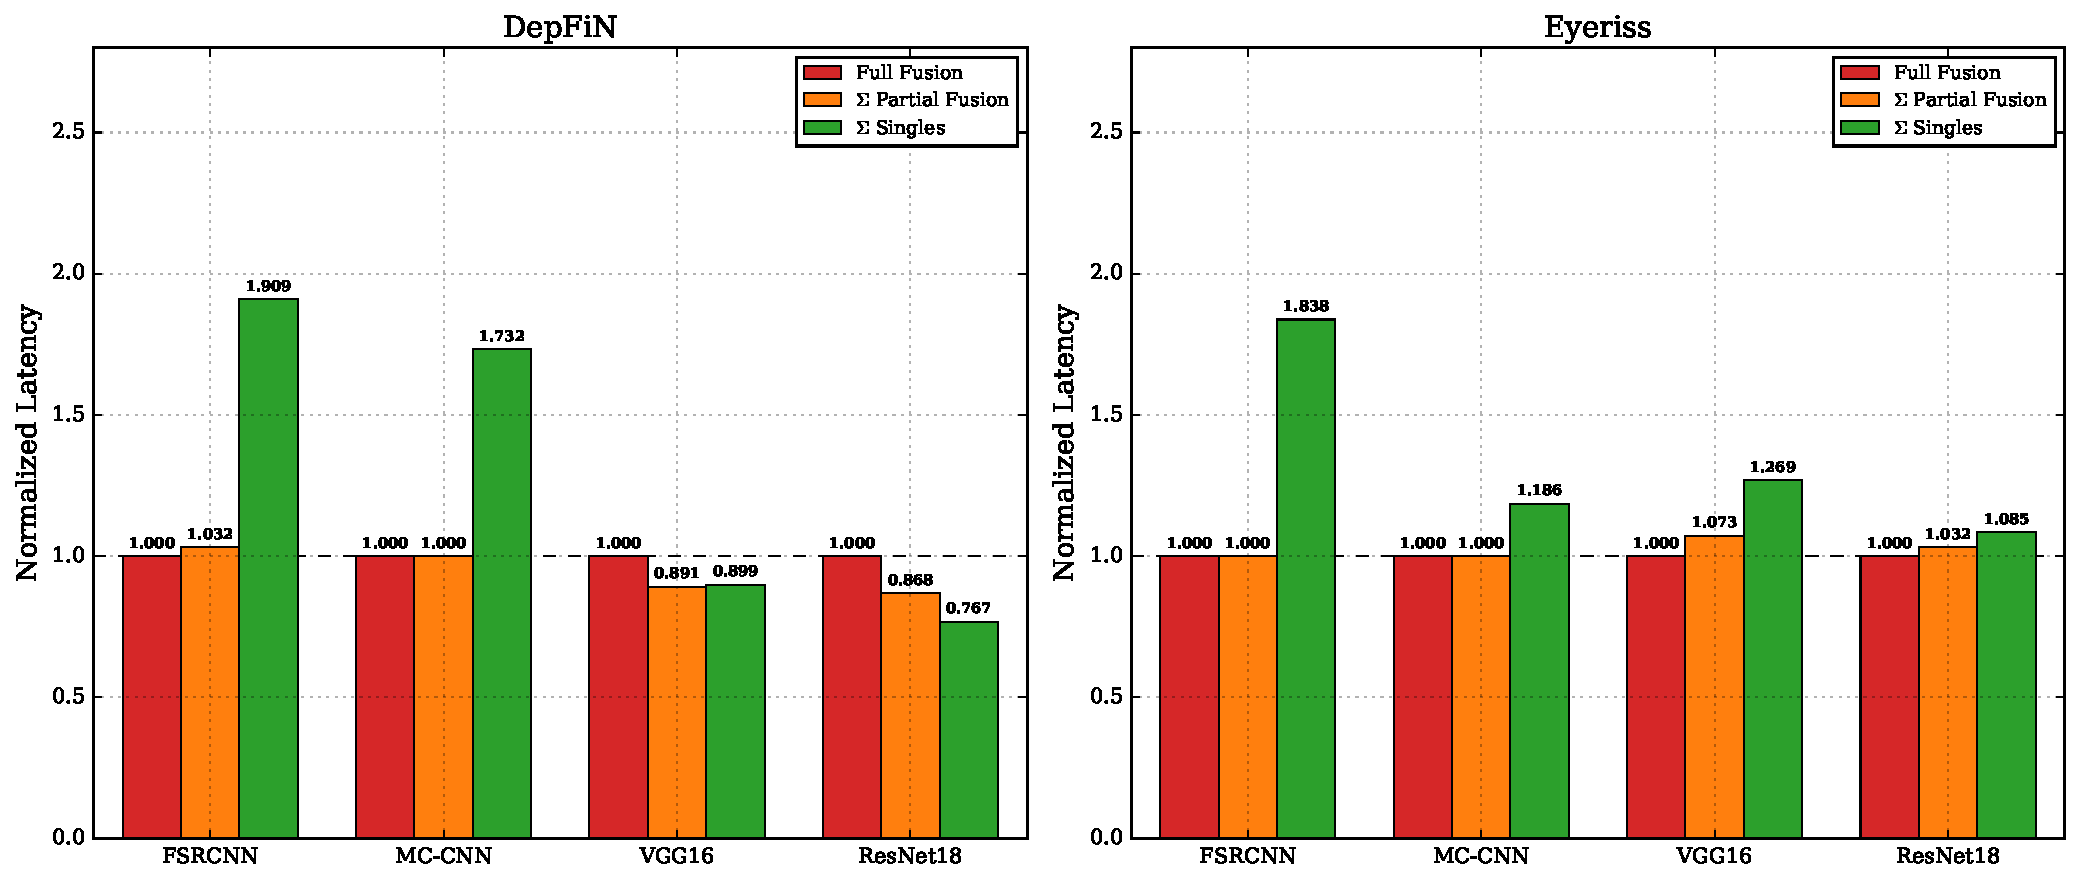
\includegraphics[width=0.95\textwidth]{plots/fusion_auto_latency_norm.pdf}
  \caption{Scenario~A: Normalized latency (Full~Fusion\,=\,1.0).
    Bars above 1.0 indicate longer latency than full fusion.}
  \label{fig:fusion-latency-norm}
\end{figure}

\begin{figure}[htbp]
  \centering
  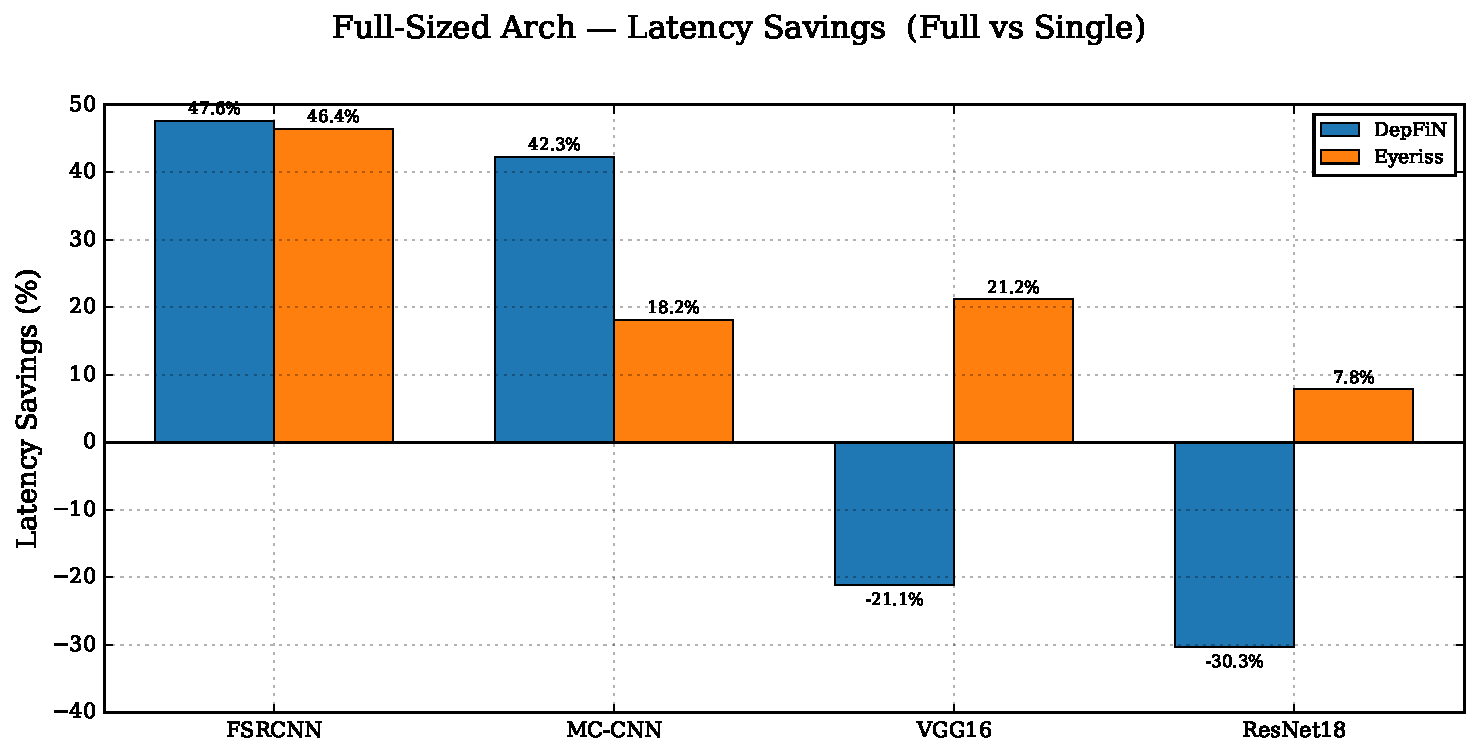
\includegraphics[width=0.75\textwidth]{plots/fusion_latency_savings.pdf}
  \caption{Scenario~A: Latency savings of full fusion relative
    to single-layer execution.
    Positive values indicate fusion is faster; negative values
    indicate fusion is slower.}
  \label{fig:fusion-latency-savings}
\end{figure}

% ── EDP ─────────────────────────────────────────────────────
\paragraph{Energy-Delay Product
  (Figure~\ref{fig:fusion-edp-norm}).}
The EDP combines energy and latency into a single efficiency
metric.

On \textbf{DepFiN}, full fusion is the clear EDP winner for the
activation-dominant workloads.
FSRCNN's single-layer EDP is $6.44\times$ the full-fusion value,
and MC-CNN is $2.31\times$: both energy and latency favor
fusion, so EDP amplifies the advantage.
For the weight-dominant workloads, however, the energy penalty of
the weight memory dominates.
VGG16 single-layer EDP is $0.035\times$ full and ResNet18 is
$0.073\times$ full.
Partial fusion occupies a middle ground: it captures most of the
latency benefit while avoiding the worst of the memory-inflation energy cost,
yielding normalized EDPs of $1.17$ (FSRCNN), $1.10$ (MC-CNN),
$0.23$ (VGG16), and $0.36$ (ResNet18).

On \textbf{Eyeriss}, the distributed register overhead shifts the
balance decisively against full fusion.
Not for FSRCNN, whose $45.6\%$ latency saving is comparable to
DepFiN's, has a full-fusion energy roughly equal to the
single-layer value ($1.02\times$), resulting in a single-layer
EDP of $1.75\times$ the full-fusion value, meaning full fusion
is still more efficient on EDP.
For MC-CNN, single-layer EDP is $0.52\times$ full, and for
VGG16 and ResNet18 it drops to $0.074\times$ and $0.13\times$,
respectively.
Partial fusion outperforms full fusion on EDP for every Eyeriss
workload, with values ranging from $0.41$ (VGG16) to $0.70$
(ResNet18).

\begin{figure}[htbp]
  \centering
  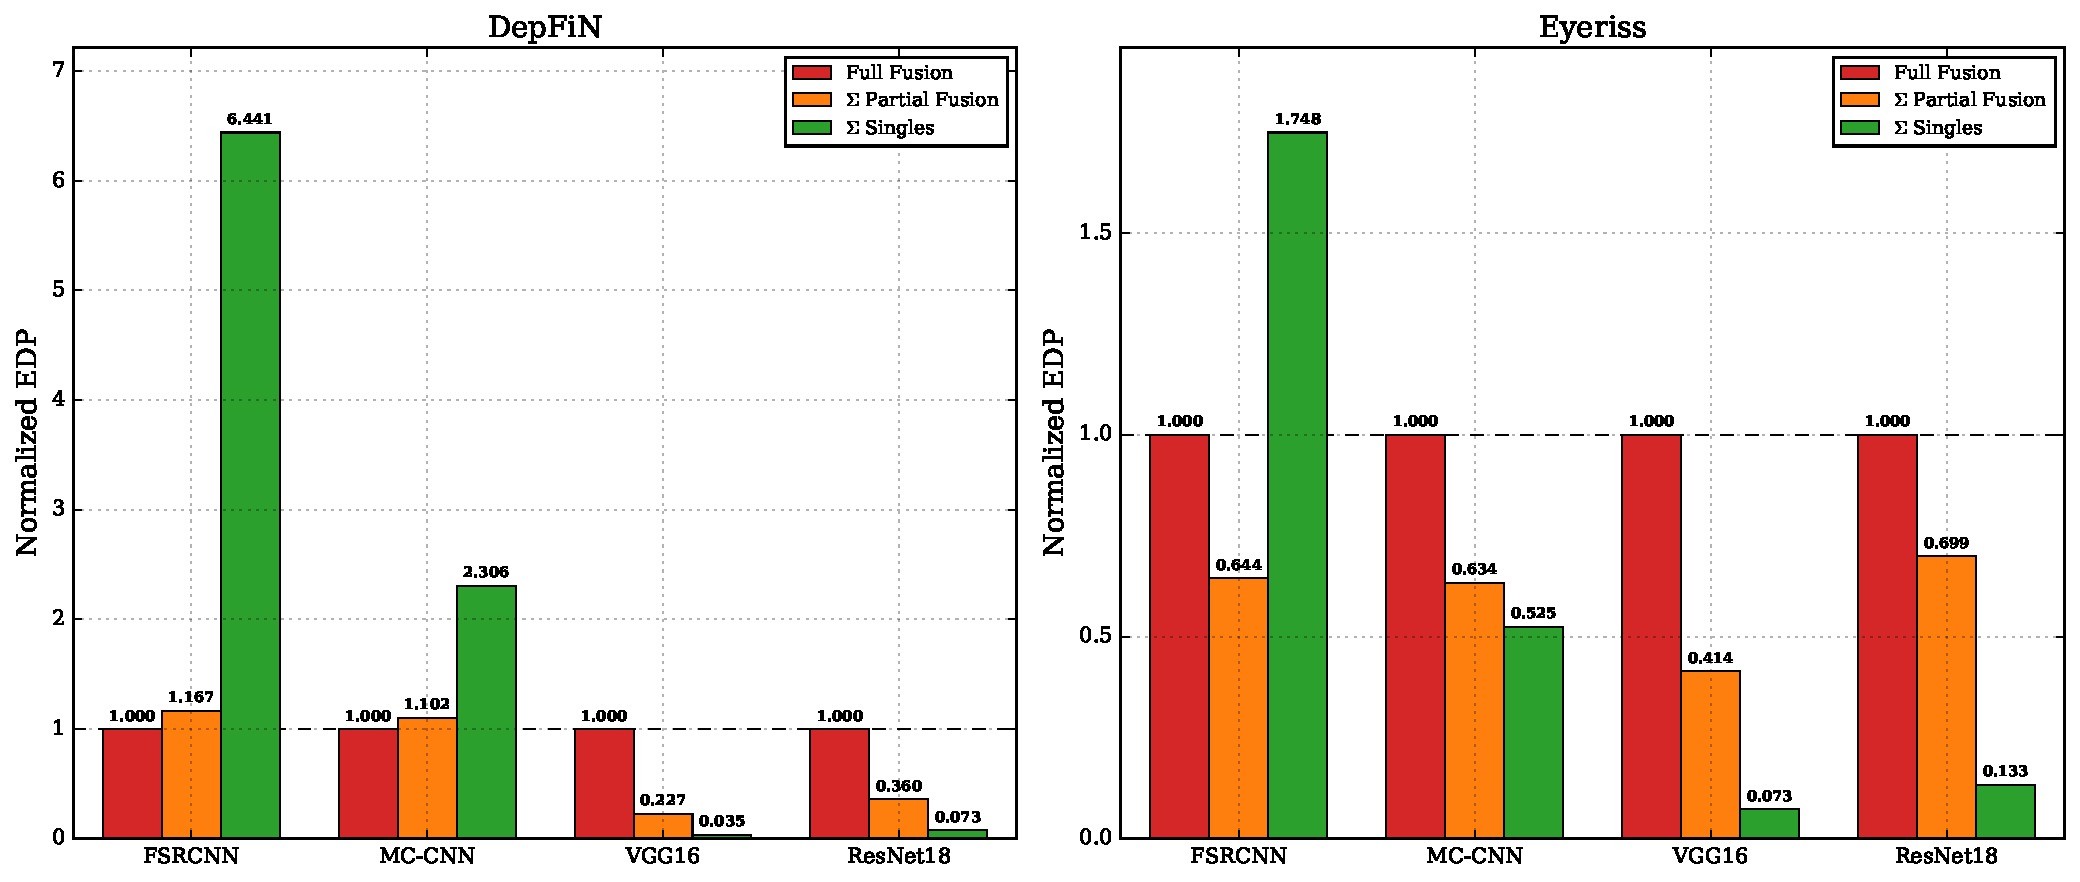
\includegraphics[width=0.95\textwidth]{plots/fusion_auto_edp_norm.pdf}
  \caption{Scenario~A: Normalized EDP (Full~Fusion\,=\,1.0).
    Bars below 1.0 indicate better efficiency than full fusion.}
  \label{fig:fusion-edp-norm}
\end{figure}

% ── DRAM Traffic ────────────────────────────────────────────
\paragraph{DRAM traffic reduction.}
\label{sec:dram-traffic}
The fundamental premise of layer fusion is the elimination of
intermediate DRAM transfers, and the data confirm that this
mechanism works as expected.
Full fusion reduces total DRAM traffic (reads + writes) by
$94.8\%$ for FSRCNN, $85.3\%$ for MC-CNN, $59.9\%$ for VGG16,
and $25.1\%$ for ResNet18, relative to single-layer execution.
These numbers are identical across the two architectures because
the DRAM access pattern depends on the tiling of the mapping, and we are trying the
same for the tile size for both the architecture for fairness of evaluation.

The reduction is largest for the activation-dominant workloads
because their intermediate activations comprise the overwhelming
majority of total DRAM traffic in single-layer mode.
For the weight-dominant workloads, weights dominate the transfer
volume, and since weights are loaded from DRAM regardless of
fusion, the relative saving is smaller.

% ── Considerations ────────────────────────────────────────────
\paragraph{Considerations.}
Full fusion achieves the elimination of
inter-layer DRAM traffic, delivering reductions of
$25$--$95\%$ depending on the workload.
This translates into significant latency improvements for
activation-dominant workloads ($42$--$48\%$ on DepFiN,
$16$--$46\%$ on Eyeriss).

The energy outcome depends on the interplay between the DRAM cost
saved and the on-chip memory overhead incurred.
At 160\,pJ\,/\,byte, full fusion is energy-beneficial on DepFiN
for activation-dominant workloads (FSRCNN, MC-CNN), where the
eliminated DRAM traffic is large and the feature memory growth is
modest.
On Eyeriss, the replicated register architecture inflates the
on-chip energy to the point where full fusion is
energy-neutral at best (FSRCNN) and energy-adverse for all other
workloads.
For weight-dominant workloads (VGG16, ResNet18), full fusion is
energy-adverse on both architectures because the massive weight
memories required for fusion drive per-access energy far above
the DRAM savings.

On EDP, full fusion wins decisively on DepFiN for the
activation-dominant workloads and marginally on Eyeriss for
FSRCNN; for all other cases, partial fusion or single-layer
execution is preferable.
The implication is that the optimal fusion strategy is
workload-dependent and architecture-dependent: activation-dominant
workloads on architectures with shared on-chip memories (DepFiN)
benefit most from aggressive fusion, while weight-dominant
workloads and architectures with replicated per-PE storage
(Eyeriss) favor partial or no fusion.
% ============================================================
%  N.3.2  Partial-Sized Architecture — Fusion Mode Comparison
% ============================================================
\subsection{Partial-Sized Architecture: Fusion Mode Comparison
  (Scenario~B)}
\label{sec:fusion-partial-sized}

\subsubsection{Motivation}

Scenario~A (Section~\ref{sec:fusion-full-sized}) sized the
architecture to support full fusion of the entire workload.
The resulting memories are large, particularly on DepFiN, where
VGG16 requires a 14.4\,MB weight memory and ResNet18 requires
10.7\,MB.
Scenario~B smaller architecture for
each workload, is large enough to fuse any two consecutive
layers, and then comparing partial-fusion execution against
single-layer execution on that same hardware.
Full fusion is not attempted, because the reduced memories
cannot accommodate it.
Table~\ref{tab:partial-sized-configs} lists the resulting
configurations.

\begin{table}[htbp]
  \centering
  \caption{Architecture configurations used for Scenario~B
    (partial-fusion-sized).
    Compared with Scenario~A
    (Table~\ref{tab:fusion-auto-configs}), the DepFiN weight
    memory shrinks substantially for the weight-dominant
    workloads, and the Eyeriss WReg drops from architecture-wide
    values to the pair-wise minimum.}
  \label{tab:partial-sized-configs}
  \begin{tabular}{ll rr rr}
    \toprule
    & & \multicolumn{2}{c}{DepFiN} & \multicolumn{2}{c}{Eyeriss} \\
    \cmidrule(lr){3-4} \cmidrule(lr){5-6}
    Workload & PEs
      & fmem & wmem
      & GB & WReg \\
    \midrule
    FSRCNN   & $16 \times 128$ / $128 \times 16$
      & 248\,KB  & 9\,KB
      & 128\,KB  & 384 \\
    MC-CNN   & $8 \times 256$\, / $256 \times 8$
      & 396\,KB  & 22\,KB
      & 128\,KB  & 384 \\
    VGG16    & $16 \times 128$ / $512 \times 32$
      & 112\,KB  & 4\,610\,KB
      & 128\,KB  & 576 \\
    ResNet18 & $16 \times 128$ / $512 \times 32$
      & 48\,KB   & 4\,608\,KB
      & 128\,KB  & 384 \\
    \bottomrule
  \end{tabular}
\end{table}

The memory reductions are conspicuous for the weight-dominant
workloads on DepFiN.
VGG16's weight memory drops from 14\,366\,KB (Scenario~A) to
4\,610\,KB, a $3.1\times$ reduction; ResNet18 drops from
10\,738\,KB to 4\,608\,KB ($2.3\times$).
On Eyeriss, VGG16's Weight Register (WReg) falls from 1\,200 to 576 bytes per PE,
and ResNet18's WReg from 902 to 384 bytes.
The activation-dominant workloads see smaller but still
meaningful reductions on DepFiN (FSRCNN Feature Memory from 576\,KB to
248\,KB, Weight Memory from 19\,KB to 9\,KB), while on Eyeriss their
configuration is unchanged because the GlobalBuffer and Weight Register
were already set at the pairwise minimum.

\subsubsection{Results}

Figure~\ref{fig:partial-sized-norm} presents the normalized
comparison (partial fusion\,=\,1.0) for energy, latency, and EDP.

\paragraph{Energy.}
On \textbf{DepFiN}, the energy outcome mirrors the
workload-type split observed in Scenario~A.
For the activation-dominant workloads, partial fusion is
\emph{cheaper} than single-layer execution: FSRCNN single-layer
energy is $3.03\times$ the partial-fusion value, and MC-CNN is
$1.21\times$.
At 160\,pJ\,/\,byte, the DRAM traffic eliminated by fusing even
two consecutive layers outweighs the per-access cost increase from
the modestly sized feature memories (248\,KB for FSRCNN, 396\,KB
for MC-CNN).
Notably, the Scenario~B partial-fusion energy is also lower than
the Scenario~A full-fusion energy in absolute terms, because the smaller
memories reduce the per-access overhead.

For the weight-dominant workloads on DepFiN, single-layer
execution remains substantially cheaper: VGG16 single costs only
$15.6\%$ of the partial-fusion energy, and ResNet18 costs
$27.7\%$.
Even though the weight memory has been reduced by $2$--$3\times$
relative to Scenario~A, 4.6\,MB is still large enough to
inflate per-access energy well above the DRAM savings.

On \textbf{Eyeriss}, partial fusion is more expensive than
single-layer execution for every workload.
FSRCNN is closest to break-even (single\,$= 0.88\times$\,partial),
while the weight-dominant workloads show larger penalties:
MC-CNN single costs $40.5\%$ of partial, VGG16 costs $12.9\%$,
and ResNet18 costs $18.1\%$.
The replicated register architecture amplifies the on-chip
overhead, as discussed in Section~\ref{sec:fusion-full-sized}.

\paragraph{Latency.}
The latency pattern mirrors Scenario~A closely.
Partial fusion saves $45.9\%$ on FSRCNN and $42.3\%$ on MC-CNN
for DepFiN, comparable to the $47.6\%$ and $42.3\%$ savings of
full fusion in Scenario~A.
On Eyeriss the activation-dominant savings are identical to
Scenario~A ($45.6\%$ for FSRCNN, $15.7\%$ for MC-CNN), because
the architecture configuration has not changed for these
workloads.

For the weight-dominant workloads the latency picture improves
relative to Scenario~A.
On DepFiN, VGG16 is now essentially latency-neutral ($+0.8\%$
saving), a marked improvement over the $-11.3\%$ penalty of
full fusion in Scenario~A, because the smaller weight memory
reduces the scheduling overhead.
ResNet18 is still slower under fusion ($-7.5\%$), but the
penalty is less severe than the $-30.3\%$ in Scenario~A.
On Eyeriss, VGG16 and ResNet18 retain the same modest savings
($15.5\%$ and $4.9\%$) observed in Scenario~A.

\paragraph{EDP.}
On \textbf{DepFiN}, partial fusion wins on EDP for both
activation-dominant workloads.
FSRCNN's single-layer EDP is $5.61\times$ the partial-fusion
value, and MC-CNN is $2.08\times$: both energy and latency
favour fusion, and EDP amplifies the advantage.
For the weight-dominant workloads, single-layer execution
dominates: VGG16 single-layer EDP is $0.157\times$ partial, and
ResNet18 is $0.257\times$ partial.

On \textbf{Eyeriss}, partial fusion wins on EDP for FSRCNN
(single\,$= 1.62\times$\,partial), where the $45.6\%$ latency
saving outweighs the modest $1.13\times$ energy penalty.
For all other Eyeriss workloads, single-layer execution wins:
MC-CNN single EDP is $0.48\times$ partial, VGG16 is
$0.15\times$, and ResNet18 is $0.19\times$.

In total, partial fusion wins on EDP in three of the eight
architecture--workload combinations (FSRCNN and MC-CNN on DepFiN,
FSRCNN on Eyeriss), compared with the equivalent three of eight
in Scenario~A.

\begin{figure}[htbp]
  \centering
  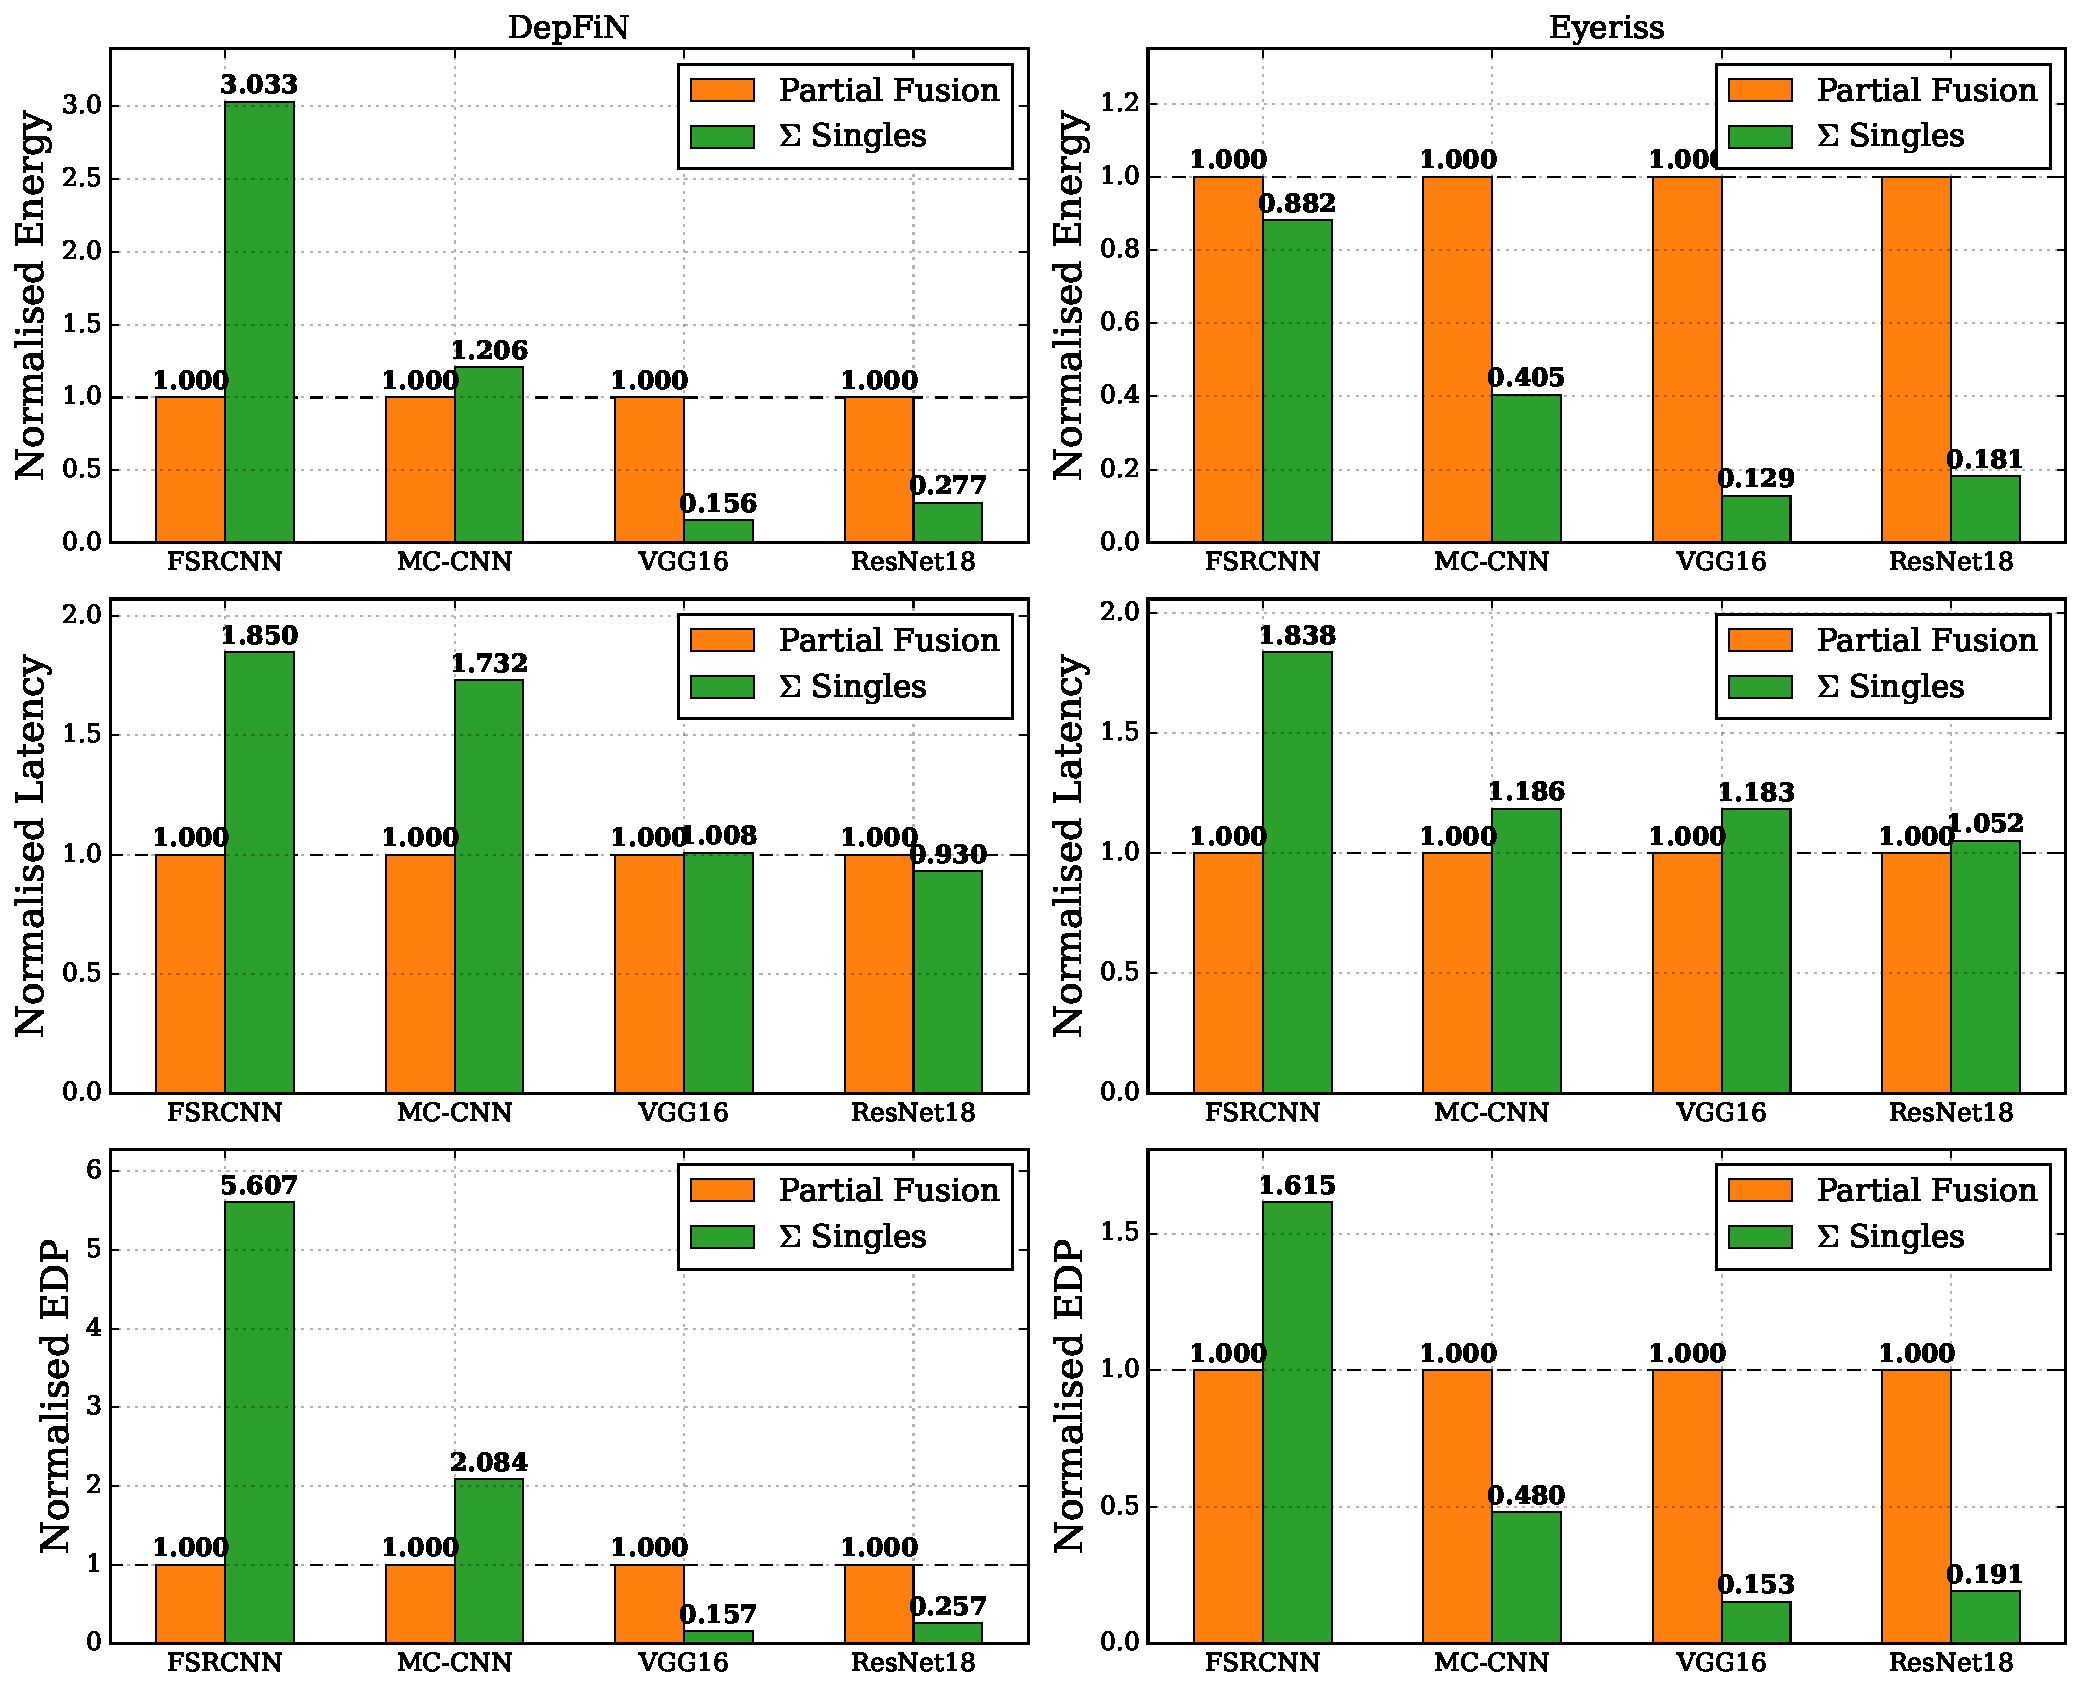
\includegraphics[width=0.95\textwidth]{plots/fusion_partial_sized_norm.pdf}
  \caption{Scenario~B — Normalised energy (top), latency (middle),
    and EDP (bottom), with partial fusion\,=\,1.0.
    Bars below 1.0 indicate the single-layer sum is more efficient.}
  \label{fig:partial-sized-norm}
\end{figure}

\paragraph{Comparison with Scenario~A.}
Scenario~B demonstrates that sizing the architecture for pairwise
fusion rather than full fusion brings two clear advantages.

The first is the substantial memory reduction
(Table~\ref{tab:partial-sized-configs}), which lowers energy cost access for the memories and registers.
The second is that the latency benefit of fusion is almost fully
preserved: partial fusion captures $96$--$100\%$ of the
full-fusion latency saving for the activation-dominant workloads,
and it eliminates or greatly reduces the worst-case latency
penalty that full fusion imposed on DepFiN
($-11.3\%{\to}+0.8\%$ for VGG16; $-30.3\%{\to}-7.5\%$ for
ResNet18).


The EDP verdict is identical in scope: three of eight
architecture--workload combinations favor fusion in both
scenarios (FSRCNN and MC-CNN on DepFiN, FSRCNN on Eyeriss).
The weight-dominant workloads continue to favor single-layer
execution on both architectures, regardless of whether the
design targets full or partial fusion.

\paragraph{Considerations}
A partial-fusion-sized architecture delivers nearly the same
latency and EDP benefit as a full-fusion architecture, at a
fraction of the memory cost.
For activation-dominant workloads on DepFiN, partial fusion
wins on energy, latency, and EDP simultaneously, making it
the strictly dominant strategy.
On Eyeriss, partial fusion wins on EDP only for the most
activation-heavy workload (FSRCNN), because the replicated
register overhead partially offsets the DRAM savings.
For weight-dominant workloads, the on-chip memory overhead of
fusion still outweighs the DRAM savings,
and single-layer execution remains the more efficient choice
on both architectures.
% ============================================================
%  N.3.3  Fixed-Config Scaling — Energy Ratio vs Register Size
% ============================================================
\subsection{Energy Ratio vs.\ Register Size
  (Eyeriss)}
\label{sec:fusion-fixed-scaling}

\subsubsection{Motivation}

Sections~\ref{sec:fusion-full-sized} and~\ref{sec:fusion-partial-sized}
compared fusion modes at a single architecture point per workload.
This case study will quantify the energy penalty of fusion in three different configuration of PE of Eyeriss, each requiring
progressively larger registers.

Two weight-dominant workloads, ResNet18 and VGG16, are examined
because they span a range of WReg values wide enough to reveal the scaling trend.
For each workload, three PE counts are tested
(16\,384, 8\,192, 4\,096), each paired with the minimum WReg determined by CS1.
The activation-dominant workloads (FSRCNN, MC-CNN) are excluded
from the sweep because they share a single WReg\,=\,384
regardless of PE count, so there is no register-size axis to
sweep.

\subsubsection{Results}

\paragraph{ResNet18 (Figure~\ref{fig:fusion-fixed-resnet18}).}
Table~\ref{tab:fusion-fixed-resnet18} reports the three
configurations.
At the largest array ($512 \times 32$, 16\,384~PEs, WReg\,=\,902)
the full-to-single energy ratio is $8.0\times$.
Halving the PE count to 8\,192 and doubling WReg to 1\,800
raises the ratio to $11.7\times$, a $1.5\times$ increase.
At 4\,096~PEs with WReg\,=\,3\,600, the ratio reaches
$19.6\times$.

\begin{table}[htbp]
  \centering
  \caption{Eyeriss fixed-config scaling for ResNet18 (Scenario~A).
    WReg is the minimum feasible value from CS1.
    Energy ratio\,=\,Full\,/\,Single.}
  \label{tab:fusion-fixed-resnet18}
  \begin{tabular}{lrrrrrr}
    \toprule
    Config & PEs & WReg
      & Full ($\mu$J) & Single ($\mu$J)
      & Ratio \\
    \midrule
    $512 \times 32$  & 16\,384 &    902
      & $2.37 \times 10^{4}$ & $2.98 \times 10^{3}$
      & $8.0\times$ \\
    $256 \times 32$  &  8\,192 &  1\,800
      & $3.25 \times 10^{4}$ & $2.78 \times 10^{3}$
      & $11.7\times$ \\
    $256 \times 16$  &  4\,096 &  3\,600
      & $5.20 \times 10^{4}$ & $2.65 \times 10^{3}$
      & $19.6\times$ \\
    \bottomrule
  \end{tabular}
\end{table}

The growth arises because two effects stack in the ratio.
First, the fused energy increases with WReg because every
register access touches a larger SRAM structure, and the
aggregate register capacity across all PEs is roughly constant
($902 \times 16{,}384 \approx 14.8$\,M~bytes at the top,
$3{,}600 \times 4{,}096 \approx 14.7$\,M at the bottom), so the
per-access cost rises while the total capacity stays flat.
Second, the single-layer energy \emph{decreases} slightly with
fewer PEs because single-layer mode does not require the
oversized WReg.
However, the single-layer shrinkage is modest (only
$5$--$13\%$ per step) because the DRAM component of single-layer
energy is substantial and PE-count-independent, leaving the
register-driven reduction as a minor effect.
The ratio growth is therefore driven primarily by the
fused-energy increase ($1.4$--$1.7\times$ per step).

\begin{figure}[htbp]
  \centering
  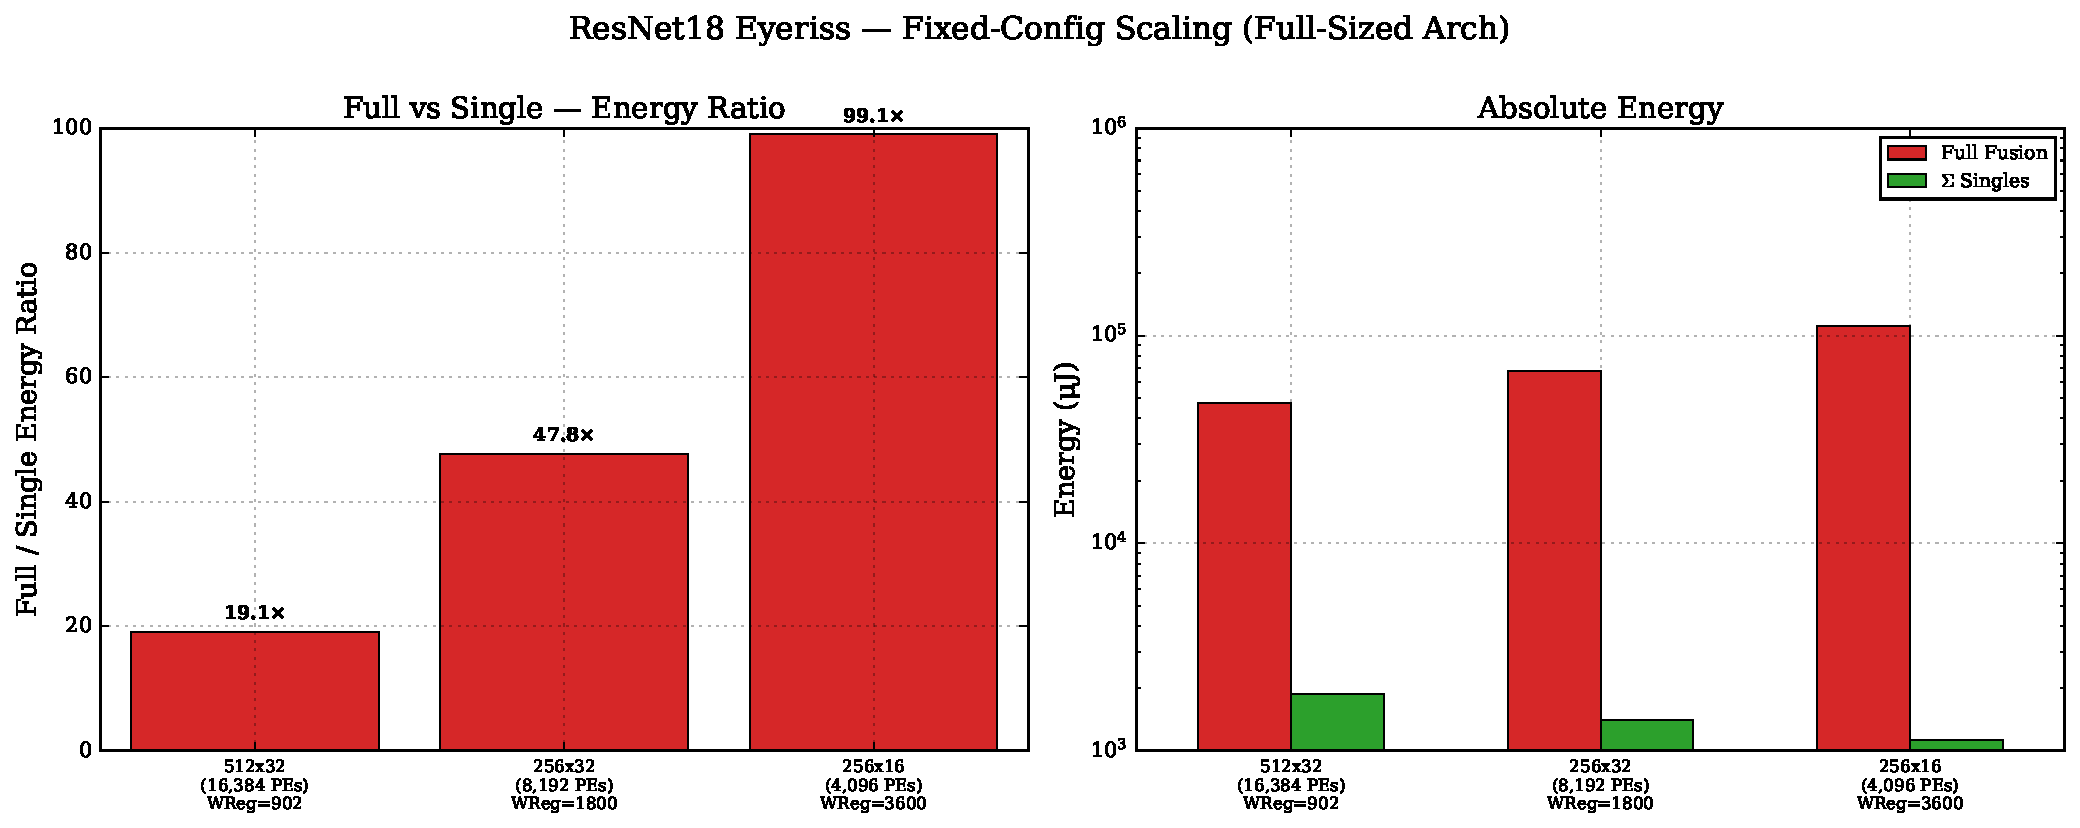
\includegraphics[width=0.95\textwidth]{plots/fusion_fixed_resnet18_scaling.pdf}
  \caption{Eyeriss fixed-config scaling for ResNet18.
    Left: full-to-single energy ratio.
    Right: absolute energy on a log scale.}
  \label{fig:fusion-fixed-resnet18}
\end{figure}

\paragraph{VGG16 (Figure~\ref{fig:fusion-fixed-vgg16}).}
VGG16 exhibits the same pattern, amplified by its larger register
requirements.
At WReg\,=\,1\,200 (16\,384~PEs) the ratio is $17.0\times$;
at WReg\,=\,2\,400 (8\,192~PEs) it rises to $28.9\times$; and at
WReg\,=\,4\,800 (4\,096~PEs) it reaches $54.1\times$.
Each doubling step grows the ratio by $1.7$--$1.9\times$,
consistent with the ResNet18 trend.

\begin{table}[htbp]
  \centering
  \caption{Eyeriss fixed-config scaling for VGG16 (Scenario~A).}
  \label{tab:fusion-fixed-vgg16}
  \begin{tabular}{lrrrrrr}
    \toprule
    Config & PEs & WReg
      & Full ($\mu$J) & Single ($\mu$J)
      & Ratio \\
    \midrule
    $512 \times 32$  & 16\,384 &  1\,200
      & $1.63 \times 10^{5}$ & $9.59 \times 10^{3}$
      & $17.0\times$ \\
    $256 \times 32$  &  8\,192 &  2\,400
      & $2.45 \times 10^{5}$ & $8.49 \times 10^{3}$
      & $28.9\times$ \\
    $256 \times 16$  &  4\,096 &  4\,800
      & $4.19 \times 10^{5}$ & $7.74 \times 10^{3}$
      & $54.1\times$ \\
    \bottomrule
  \end{tabular}
\end{table}

VGG16 also reveals a difference between full and partial fusion.
The full-to-partial energy ratio is $2.55\times$ at
WReg\,=\,1\,200 and decreases to $1.41\times$ at
WReg\,=\,4\,800, indicating that as registers grow, partial
fusion captures most of the fused-mode overhead and the gap
between the two modes narrows.
For ResNet18 the full-to-partial ratio ranges from $1.44\times$
at the smallest WReg down to $1.02\times$ at the largest,
showing near-equivalent energy for full and partial fusion at
large registers.

\begin{figure}[htbp]
  \centering
  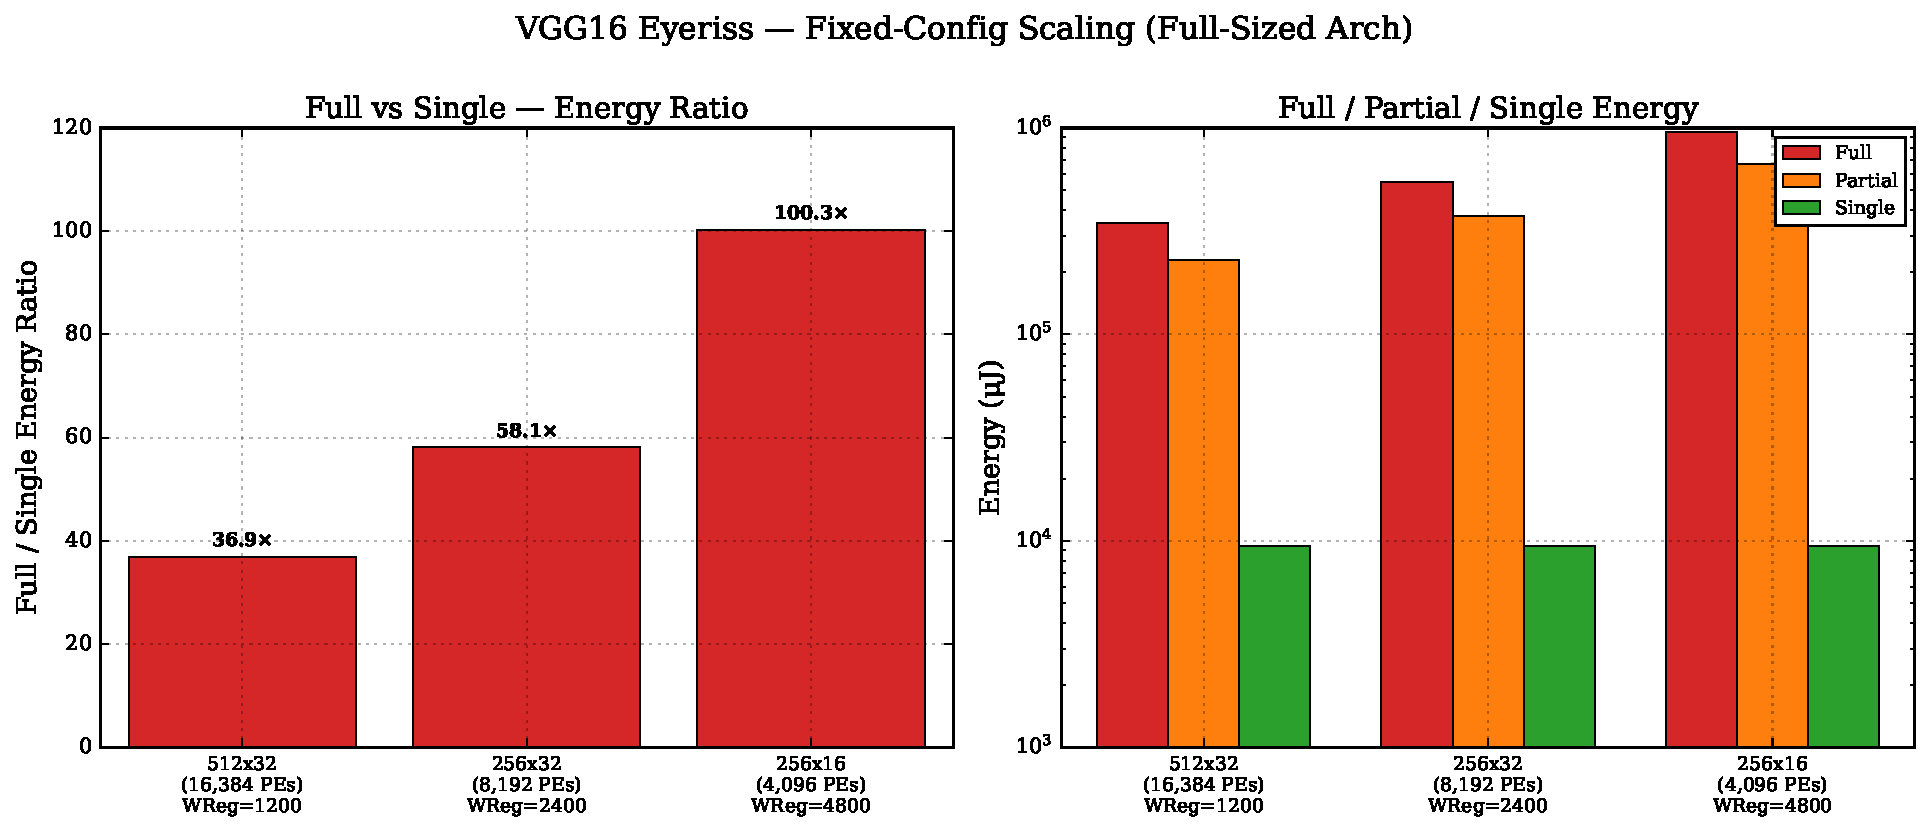
\includegraphics[width=0.95\textwidth]{plots/fusion_fixed_vgg16_scaling.pdf}
  \caption{Eyeriss fixed-config scaling for VGG16.
    Left: full-to-single energy ratio.
    Right: absolute energy (full, partial, single) on a log scale.}
  \label{fig:fusion-fixed-vgg16}
\end{figure}

\paragraph{Activation-dominant workloads.}
FSRCNN and MC-CNN do not participate in this sweep because their
WReg remains at 384~bytes regardless of the PE configuration.
At that single operating point, the full-to-single energy ratios
are $1.0\times$ (FSRCNN) and $2.2\times$ (MC-CNN), which
sit well below the weight-dominant ratios.
For FSRCNN, fusion incurs essentially no energy overhead: almost
all energy is spent in DRAM transfers that are common to both
modes.
The constant WReg reflects the fact that, for shallow networks
with small filter counts, the per-PE weight footprint is already
negligible at the minimum PE count.

\paragraph{Scaling rule.}
Across both workloads, each $2\times$ increase in WReg raises
the fusion-to-single energy ratio by a factor of roughly
$1.5$--$1.9\times$.
The fused energy grows by $1.4$--$1.7\times$ per WReg step
because each register access touches a larger SRAM structure.
The single-layer energy shrinks only modestly, by
$1.05$--$1.13\times$, because the DRAM component of single-layer
energy is substantial and PE-count-independent, so the
register-driven shrinkage is a minor effect.
The product of these two factors yields the observed
${\sim}1.5$--$1.9\times$ ratio growth per step.

\paragraph{Considerations}
The energy penalty of fusion on the Eyeriss architecture is not a
fixed constant; it \emph{scales super-linearly} with register size.
A designer who chooses a smaller PE array to save area will face a
correspondingly larger WReg and, consequently, a worse
fusion-to-single energy ratio.
At the extreme tested point (VGG16, WReg\,=\,4\,800), fusion
consumes $54\times$ the energy of single-layer execution.
This scaling behavior reinforces the conclusion from
Sections~\ref{sec:fusion-full-sized}
and~\ref{sec:fusion-partial-sized}: fusion's energy cost is
the dominant factor in the EDP trade-off, and it grows worse
as the architecture is scaled down.